\documentclass[]{book}
\usepackage{lmodern}
\usepackage{amssymb,amsmath}
\usepackage{ifxetex,ifluatex}
\usepackage{fixltx2e} % provides \textsubscript
\ifnum 0\ifxetex 1\fi\ifluatex 1\fi=0 % if pdftex
  \usepackage[T1]{fontenc}
  \usepackage[utf8]{inputenc}
\else % if luatex or xelatex
  \ifxetex
    \usepackage{mathspec}
  \else
    \usepackage{fontspec}
  \fi
  \defaultfontfeatures{Ligatures=TeX,Scale=MatchLowercase}
\fi
% use upquote if available, for straight quotes in verbatim environments
\IfFileExists{upquote.sty}{\usepackage{upquote}}{}
% use microtype if available
\IfFileExists{microtype.sty}{%
\usepackage{microtype}
\UseMicrotypeSet[protrusion]{basicmath} % disable protrusion for tt fonts
}{}
\usepackage{hyperref}
\hypersetup{unicode=true,
            pdftitle={Hitchhiker's Guide to the Tidyverse},
            pdfauthor={Cory Lanker},
            pdfborder={0 0 0},
            breaklinks=true}
\urlstyle{same}  % don't use monospace font for urls
\usepackage{natbib}
\bibliographystyle{apalike}
\usepackage{color}
\usepackage{fancyvrb}
\newcommand{\VerbBar}{|}
\newcommand{\VERB}{\Verb[commandchars=\\\{\}]}
\DefineVerbatimEnvironment{Highlighting}{Verbatim}{commandchars=\\\{\}}
% Add ',fontsize=\small' for more characters per line
\usepackage{framed}
\definecolor{shadecolor}{RGB}{248,248,248}
\newenvironment{Shaded}{\begin{snugshade}}{\end{snugshade}}
\newcommand{\KeywordTok}[1]{\textcolor[rgb]{0.13,0.29,0.53}{\textbf{#1}}}
\newcommand{\DataTypeTok}[1]{\textcolor[rgb]{0.13,0.29,0.53}{#1}}
\newcommand{\DecValTok}[1]{\textcolor[rgb]{0.00,0.00,0.81}{#1}}
\newcommand{\BaseNTok}[1]{\textcolor[rgb]{0.00,0.00,0.81}{#1}}
\newcommand{\FloatTok}[1]{\textcolor[rgb]{0.00,0.00,0.81}{#1}}
\newcommand{\ConstantTok}[1]{\textcolor[rgb]{0.00,0.00,0.00}{#1}}
\newcommand{\CharTok}[1]{\textcolor[rgb]{0.31,0.60,0.02}{#1}}
\newcommand{\SpecialCharTok}[1]{\textcolor[rgb]{0.00,0.00,0.00}{#1}}
\newcommand{\StringTok}[1]{\textcolor[rgb]{0.31,0.60,0.02}{#1}}
\newcommand{\VerbatimStringTok}[1]{\textcolor[rgb]{0.31,0.60,0.02}{#1}}
\newcommand{\SpecialStringTok}[1]{\textcolor[rgb]{0.31,0.60,0.02}{#1}}
\newcommand{\ImportTok}[1]{#1}
\newcommand{\CommentTok}[1]{\textcolor[rgb]{0.56,0.35,0.01}{\textit{#1}}}
\newcommand{\DocumentationTok}[1]{\textcolor[rgb]{0.56,0.35,0.01}{\textbf{\textit{#1}}}}
\newcommand{\AnnotationTok}[1]{\textcolor[rgb]{0.56,0.35,0.01}{\textbf{\textit{#1}}}}
\newcommand{\CommentVarTok}[1]{\textcolor[rgb]{0.56,0.35,0.01}{\textbf{\textit{#1}}}}
\newcommand{\OtherTok}[1]{\textcolor[rgb]{0.56,0.35,0.01}{#1}}
\newcommand{\FunctionTok}[1]{\textcolor[rgb]{0.00,0.00,0.00}{#1}}
\newcommand{\VariableTok}[1]{\textcolor[rgb]{0.00,0.00,0.00}{#1}}
\newcommand{\ControlFlowTok}[1]{\textcolor[rgb]{0.13,0.29,0.53}{\textbf{#1}}}
\newcommand{\OperatorTok}[1]{\textcolor[rgb]{0.81,0.36,0.00}{\textbf{#1}}}
\newcommand{\BuiltInTok}[1]{#1}
\newcommand{\ExtensionTok}[1]{#1}
\newcommand{\PreprocessorTok}[1]{\textcolor[rgb]{0.56,0.35,0.01}{\textit{#1}}}
\newcommand{\AttributeTok}[1]{\textcolor[rgb]{0.77,0.63,0.00}{#1}}
\newcommand{\RegionMarkerTok}[1]{#1}
\newcommand{\InformationTok}[1]{\textcolor[rgb]{0.56,0.35,0.01}{\textbf{\textit{#1}}}}
\newcommand{\WarningTok}[1]{\textcolor[rgb]{0.56,0.35,0.01}{\textbf{\textit{#1}}}}
\newcommand{\AlertTok}[1]{\textcolor[rgb]{0.94,0.16,0.16}{#1}}
\newcommand{\ErrorTok}[1]{\textcolor[rgb]{0.64,0.00,0.00}{\textbf{#1}}}
\newcommand{\NormalTok}[1]{#1}
\usepackage{longtable,booktabs}
\usepackage{graphicx,grffile}
\makeatletter
\def\maxwidth{\ifdim\Gin@nat@width>\linewidth\linewidth\else\Gin@nat@width\fi}
\def\maxheight{\ifdim\Gin@nat@height>\textheight\textheight\else\Gin@nat@height\fi}
\makeatother
% Scale images if necessary, so that they will not overflow the page
% margins by default, and it is still possible to overwrite the defaults
% using explicit options in \includegraphics[width, height, ...]{}
\setkeys{Gin}{width=\maxwidth,height=\maxheight,keepaspectratio}
\IfFileExists{parskip.sty}{%
\usepackage{parskip}
}{% else
\setlength{\parindent}{0pt}
\setlength{\parskip}{6pt plus 2pt minus 1pt}
}
\setlength{\emergencystretch}{3em}  % prevent overfull lines
\providecommand{\tightlist}{%
  \setlength{\itemsep}{0pt}\setlength{\parskip}{0pt}}
\setcounter{secnumdepth}{5}
% Redefines (sub)paragraphs to behave more like sections
\ifx\paragraph\undefined\else
\let\oldparagraph\paragraph
\renewcommand{\paragraph}[1]{\oldparagraph{#1}\mbox{}}
\fi
\ifx\subparagraph\undefined\else
\let\oldsubparagraph\subparagraph
\renewcommand{\subparagraph}[1]{\oldsubparagraph{#1}\mbox{}}
\fi

%%% Use protect on footnotes to avoid problems with footnotes in titles
\let\rmarkdownfootnote\footnote%
\def\footnote{\protect\rmarkdownfootnote}

%%% Change title format to be more compact
\usepackage{titling}

% Create subtitle command for use in maketitle
\providecommand{\subtitle}[1]{
  \posttitle{
    \begin{center}\large#1\end{center}
    }
}

\setlength{\droptitle}{-2em}

  \title{Hitchhiker's Guide to the Tidyverse}
    \pretitle{\vspace{\droptitle}\centering\huge}
  \posttitle{\par}
    \author{Cory Lanker}
    \preauthor{\centering\large\emph}
  \postauthor{\par}
      \predate{\centering\large\emph}
  \postdate{\par}
    \date{2019-07-22}

\usepackage{booktabs}
\usepackage{amsthm}
\makeatletter
\def\thm@space@setup{%
  \thm@preskip=8pt plus 2pt minus 4pt
  \thm@postskip=\thm@preskip
}
\makeatother

\begin{document}
\maketitle

{
\setcounter{tocdepth}{1}
\tableofcontents
}
\chapter*{Introduction}\label{introduction}
\addcontentsline{toc}{chapter}{Introduction}

Introducing the tidyverse with two data sets:

\begin{enumerate}
\def\labelenumi{\arabic{enumi}.}
\tightlist
\item
  Basic plots with \texttt{tibble} and \texttt{ggplot2} using
  \texttt{Boston} house prices.
\item
  Preprocessing with \texttt{tidyr} and \texttt{dplyr} using
  \texttt{Lahman} baseball data.
\end{enumerate}

Though some of these commands will be used, we won't go deeply into the
following tidyverse packages:

\begin{enumerate}
\def\labelenumi{\arabic{enumi}.}
\tightlist
\item
  Reading in data with \texttt{readr}.
\item
  String manipulation with \texttt{stringr}.
\item
  Dates and times with \texttt{lubridate}.
\item
  Handling factors with \texttt{forcats}.
\end{enumerate}

R proficiency is assumed. These notes aim to bring a functional R coder
into the tidyverse realm.

\begin{Shaded}
\begin{Highlighting}[]
\CommentTok{# To install the necessary packages in the tidyverse:}
\KeywordTok{install.packages}\NormalTok{(}\StringTok{"tidyverse"}\NormalTok{, }\DataTypeTok{dependencies =} \OtherTok{TRUE}\NormalTok{)}
\end{Highlighting}
\end{Shaded}

This document is built with R Markdown, \textbf{knitr} \citep{xie2015},
and the \textbf{bookdown} package \citep{R-bookdown}.

\chapter{\texorpdfstring{tibbles, ggplot2, and the
\emph{tidyverse}}{tibbles, ggplot2, and the tidyverse}}\label{ch:intro}

The tidyverse universe includes:

In general, the tidyverse is the following:

\begin{enumerate}
\def\labelenumi{\arabic{enumi}.}
\tightlist
\item
  provided the \texttt{pipe} command \texttt{\%\textgreater{}\%}
\end{enumerate}

\begin{itemize}
\tightlist
\item
  \texttt{x\ \%\textgreater{}\%\ f(y,\ z,\ ...)} is
  \texttt{f(x,\ y,\ z,\ ...)}
\item
  allows chained commands for better coherence
\item
  e.g., \texttt{mtcars\ \%\textgreater{}\%\ apply(2,\ mean)} is error
  without \texttt{tidyr::\%\textgreater{}\%}
\end{itemize}

\begin{enumerate}
\def\labelenumi{\arabic{enumi}.}
\setcounter{enumi}{1}
\tightlist
\item
  \texttt{tibble} is the improved data structure of the tidyverse
\end{enumerate}

\begin{itemize}
\tightlist
\item
  easier to read-in data to a useful format
\item
  automatic type conversion
\item
  nicer printing options
\end{itemize}

\begin{enumerate}
\def\labelenumi{\arabic{enumi}.}
\setcounter{enumi}{2}
\tightlist
\item
  \texttt{dplyr} provides tibble manipulation commands
\end{enumerate}

\begin{itemize}
\tightlist
\item
  understandable data processing with \texttt{pipe} streams
\item
  \textbf{filter} data faster
\item
  \textbf{arrange} rows of data easily
\item
  \textbf{select} columns quickly
\item
  \textbf{mutate} variables
\item
  \textbf{summarize} according to \texttt{group\_by()}
\item
  also provides SQL relational operations
\end{itemize}

\begin{enumerate}
\def\labelenumi{\arabic{enumi}.}
\setcounter{enumi}{3}
\tightlist
\item
  \texttt{ggplot2} is a plotting syntax (grammar of graphics)
\end{enumerate}

\begin{itemize}
\tightlist
\item
  \texttt{qplot()} provides a sensible \textbf{q}uick \textbf{plot}
\item
  apply plot types to data rather than the reverse
\item
  e.g.
  \texttt{ggplot(data)\ +\ plot\_type(aes(xvar,\ yvar,\ groups),\ options)}
\item
  allows grid of plots by group using \textbf{facets}
\item
  overlays statistical summaries, e.g. \texttt{+\ geom\_smooth(x,\ y)}
\item
  ``add'' options such as transformed axes, labels, coordinates, etc.
\end{itemize}

\begin{enumerate}
\def\labelenumi{\arabic{enumi}.}
\setcounter{enumi}{4}
\tightlist
\item
  \texttt{readr} is a faster, less painful read-in method
\end{enumerate}

\begin{itemize}
\tightlist
\item
  \texttt{read\_fun} denotes \texttt{readr} functions (instead of
  \texttt{read.fun})
\item
  guesses column types
\item
  offers writing functions, too
\item
  allows read and write with RDS, R's binary format
\end{itemize}

\begin{enumerate}
\def\labelenumi{\arabic{enumi}.}
\setcounter{enumi}{5}
\tightlist
\item
  \texttt{tidyr} recharacterizes tibbles
\end{enumerate}

\begin{itemize}
\tightlist
\item
  \texttt{spread()} turns key and value columns into key-category
  columns
\item
  e.g., \texttt{state,\ year,\ pop} into
  \texttt{state,\ 1990,\ 1991,\ ...} of pop values
\item
  \texttt{gather()} turns expands data frames by condensing columns
\item
  e.g., condenses \texttt{1990,\ 1991,\ ...} into two
  \texttt{year,\ pop} columns
\end{itemize}

\begin{enumerate}
\def\labelenumi{\arabic{enumi}.}
\setcounter{enumi}{6}
\tightlist
\item
  Other helpful tidyverse packages:
\end{enumerate}

\begin{itemize}
\tightlist
\item
  \texttt{stringr} offers many useful \texttt{str\_fun} operations
\item
  \texttt{forcats} has operations \_for cat\_egorical variables
\item
  \texttt{lubridate} provides date and time control
\item
  \texttt{purrr}
\end{itemize}

The examples I'll use is the Boston housing database and the Lahman
baseball database. By doing analysis on these two data sets, I hope to
introduce the power of the tidyverse.

\section{Tibbles: Boston housing
data}\label{tibbles-boston-housing-data}

Load, convert, print a tibble.

\begin{Shaded}
\begin{Highlighting}[]
\CommentTok{# Convert to a tibble so it prints nicely}
\KeywordTok{library}\NormalTok{(MASS)}
\NormalTok{select <-}\StringTok{ }\NormalTok{dplyr}\OperatorTok{::}\NormalTok{select}
\NormalTok{boston <-}\StringTok{ }\KeywordTok{as_tibble}\NormalTok{(MASS}\OperatorTok{::}\NormalTok{Boston)}
\NormalTok{boston}
\end{Highlighting}
\end{Shaded}

\begin{verbatim}
## # A tibble: 506 x 14
##       crim    zn indus  chas   nox    rm   age   dis   rad   tax ptratio
##      <dbl> <dbl> <dbl> <int> <dbl> <dbl> <dbl> <dbl> <int> <dbl>   <dbl>
##  1 0.00632  18    2.31     0 0.538  6.58  65.2  4.09     1   296    15.3
##  2 0.0273    0    7.07     0 0.469  6.42  78.9  4.97     2   242    17.8
##  3 0.0273    0    7.07     0 0.469  7.18  61.1  4.97     2   242    17.8
##  4 0.0324    0    2.18     0 0.458  7.00  45.8  6.06     3   222    18.7
##  5 0.0690    0    2.18     0 0.458  7.15  54.2  6.06     3   222    18.7
##  6 0.0298    0    2.18     0 0.458  6.43  58.7  6.06     3   222    18.7
##  7 0.0883   12.5  7.87     0 0.524  6.01  66.6  5.56     5   311    15.2
##  8 0.145    12.5  7.87     0 0.524  6.17  96.1  5.95     5   311    15.2
##  9 0.211    12.5  7.87     0 0.524  5.63 100    6.08     5   311    15.2
## 10 0.170    12.5  7.87     0 0.524  6.00  85.9  6.59     5   311    15.2
## # ... with 496 more rows, and 3 more variables: black <dbl>, lstat <dbl>,
## #   medv <dbl>
\end{verbatim}

\begin{Shaded}
\begin{Highlighting}[]
\NormalTok{?MASS}\OperatorTok{::}\NormalTok{Boston}
\end{Highlighting}
\end{Shaded}

\begin{itemize}
\tightlist
\item
  crim per capita crime rate by town.
\item
  zn proportion of residential land zoned for lots over 25,000 sq.ft.
\item
  indus proportion of non-retail business acres per town.
\item
  chas Charles River dummy variable (= 1 if tract bounds river; 0
  otherwise).
\item
  nox nitrogen oxides concentration (parts per 10 million).
\item
  rm average number of rooms per dwelling.
\item
  age proportion of owner-occupied units built prior to 1940.
\item
  dis weighted mean of distances to five Boston employment centres.
\item
  rad index of accessibility to radial highways.
\item
  tax full-value property-tax rate per \$10,000.
\item
  ptratio pupil-teacher ratio by town.
\item
  black \(1000(Bk - 0.63)^2\) where Bk is the proportion of blacks by
  town.
\item
  lstat lower status of the population (percent).
\item
  medv median value of owner-occupied homes in \$1000s.
\end{itemize}

A ggplot is the first declaration (usually variable \texttt{data} is
defined), followed by graphics definitions (operations on the data):

\begin{Shaded}
\begin{Highlighting}[]
\KeywordTok{ggplot}\NormalTok{(}\DataTypeTok{data =}\NormalTok{ boston) }\OperatorTok{+}\StringTok{ }
\StringTok{  }\KeywordTok{geom_point}\NormalTok{(}\DataTypeTok{mapping =} \KeywordTok{aes}\NormalTok{(}\DataTypeTok{x =}\NormalTok{ rm, }\DataTypeTok{y =}\NormalTok{ medv), }\DataTypeTok{alpha=}\FloatTok{0.4}\NormalTok{) }\OperatorTok{+}
\StringTok{  }\KeywordTok{labs}\NormalTok{(}\DataTypeTok{x =} \StringTok{"avg. rooms per house"}\NormalTok{,}
       \DataTypeTok{y =} \StringTok{"median house value"}\NormalTok{,}
       \DataTypeTok{title =} \StringTok{"House values vs. size in Boston"}\NormalTok{)}
\end{Highlighting}
\end{Shaded}

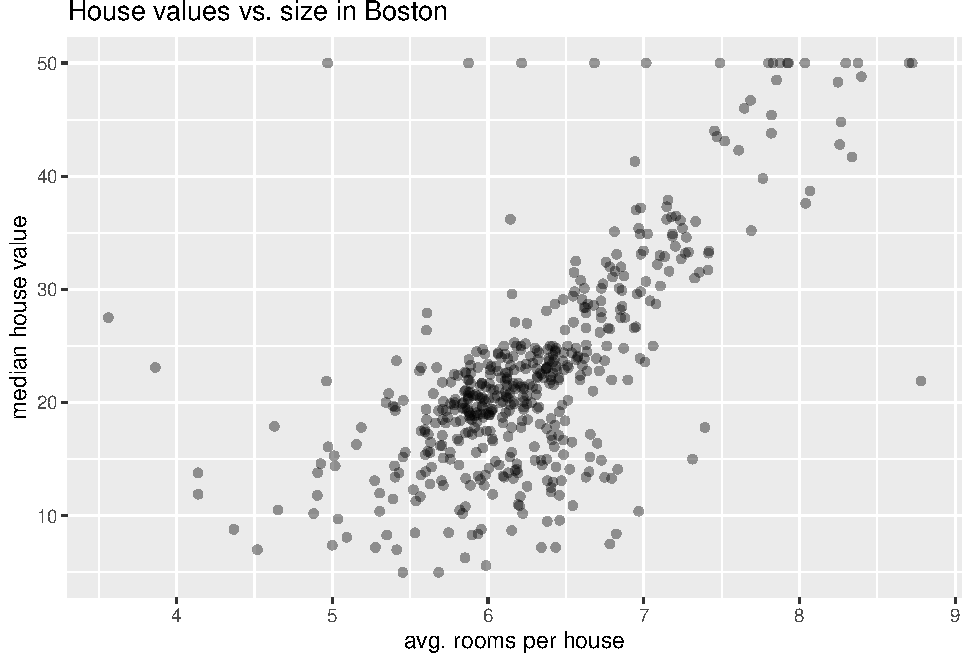
\includegraphics{tidyverse-class_files/figure-latex/price-rooms-1-1.pdf}

Making a histogram of all numeric variables. First step, gather all
variables.

\begin{Shaded}
\begin{Highlighting}[]
\NormalTok{boston }\OperatorTok
\StringTok{  }\KeywordTok{keep}\NormalTok{(is.numeric) }\OperatorTok\StringTok{  }\CommentTok{# strips all non-numeric columns (unnecessary here)}
\StringTok{  }\KeywordTok{gather}\NormalTok{()  }\CommentTok{# puts all variable values in a single column 'value'}
\end{Highlighting}
\end{Shaded}

\begin{verbatim}
## # A tibble: 7,084 x 2
##    key     value
##    <chr>   <dbl>
##  1 crim  0.00632
##  2 crim  0.0273 
##  3 crim  0.0273 
##  4 crim  0.0324 
##  5 crim  0.0690 
##  6 crim  0.0298 
##  7 crim  0.0883 
##  8 crim  0.145  
##  9 crim  0.211  
## 10 crim  0.170  
## # ... with 7,074 more rows
\end{verbatim}

Facet wrap allows plotting each \texttt{key} level separately.

\begin{Shaded}
\begin{Highlighting}[]
\NormalTok{boston }\OperatorTok\StringTok{ }
\StringTok{  }\KeywordTok{gather}\NormalTok{() }\OperatorTok
\StringTok{  }\KeywordTok{ggplot}\NormalTok{() }\OperatorTok{+}
\StringTok{    }\KeywordTok{facet_wrap}\NormalTok{(}\OperatorTok{~}\StringTok{ }\NormalTok{key, }\DataTypeTok{scales =} \StringTok{"free"}\NormalTok{) }\OperatorTok{+}
\StringTok{    }\KeywordTok{geom_histogram}\NormalTok{(}\DataTypeTok{mapping =} \KeywordTok{aes}\NormalTok{(value), }\DataTypeTok{bins=}\DecValTok{20}\NormalTok{)}
\end{Highlighting}
\end{Shaded}

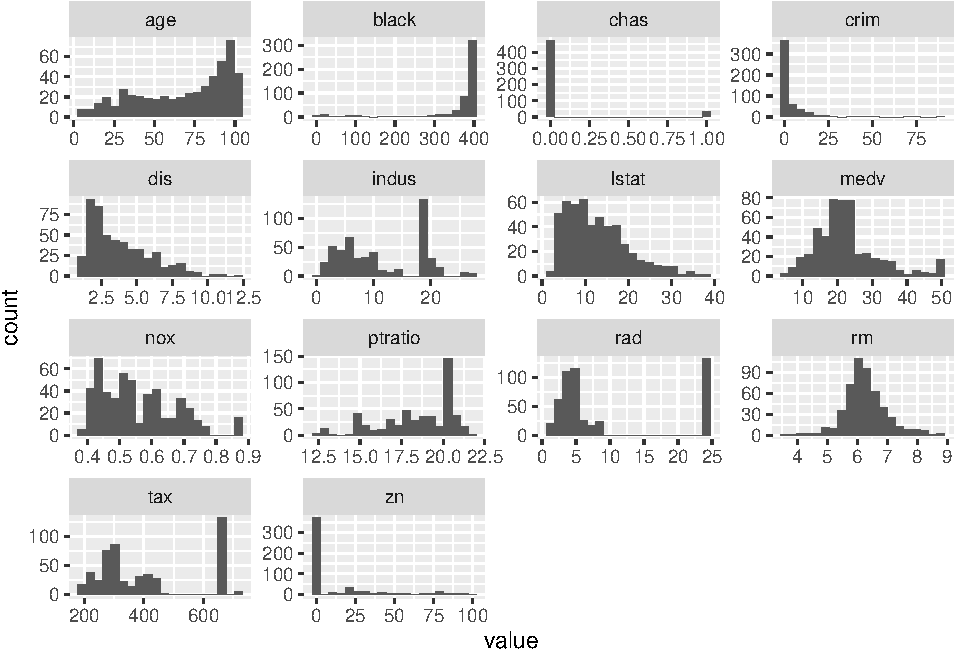
\includegraphics{tidyverse-class_files/figure-latex/all-var-hist-1.pdf}

From the histograms, there seems to be only a few values of
\texttt{crim} over 30.

\begin{Shaded}
\begin{Highlighting}[]
\NormalTok{boston }\OperatorTok
\StringTok{  }\KeywordTok{filter}\NormalTok{(crim }\OperatorTok{>}\StringTok{ }\DecValTok{30}\NormalTok{)}
\end{Highlighting}
\end{Shaded}

\begin{verbatim}
## # A tibble: 8 x 14
##    crim    zn indus  chas   nox    rm   age   dis   rad   tax ptratio black
##   <dbl> <dbl> <dbl> <int> <dbl> <dbl> <dbl> <dbl> <int> <dbl>   <dbl> <dbl>
## 1  89.0     0  18.1     0 0.671  6.97  91.9  1.42    24   666    20.2 397. 
## 2  38.4     0  18.1     0 0.693  5.45 100    1.49    24   666    20.2 397. 
## 3  41.5     0  18.1     0 0.693  5.53  85.4  1.61    24   666    20.2 329. 
## 4  67.9     0  18.1     0 0.693  5.68 100    1.43    24   666    20.2 385. 
## 5  51.1     0  18.1     0 0.597  5.76 100    1.41    24   666    20.2   2.6
## 6  45.7     0  18.1     0 0.693  4.52 100    1.66    24   666    20.2  88.3
## 7  73.5     0  18.1     0 0.679  5.96 100    1.80    24   666    20.2  16.4
## 8  37.7     0  18.1     0 0.679  6.20  78.7  1.86    24   666    20.2  18.8
## # ... with 2 more variables: lstat <dbl>, medv <dbl>
\end{verbatim}

\section{ggplot2 and EDA}\label{ggplot2-and-eda}

But we want to know the conditional distributions according to
\texttt{medv}. First, showing this with conditional densities.

\begin{Shaded}
\begin{Highlighting}[]
\NormalTok{boston }\OperatorTok\StringTok{ }
\StringTok{  }\KeywordTok{gather}\NormalTok{(}\StringTok{'key'}\NormalTok{, }\StringTok{'value'}\NormalTok{, }\OperatorTok{-}\KeywordTok{one_of}\NormalTok{(}\StringTok{'medv'}\NormalTok{)) }\OperatorTok
\StringTok{  }\KeywordTok{mutate}\NormalTok{(}\DataTypeTok{price_gr =} \KeywordTok{ntile}\NormalTok{(medv, }\DecValTok{4}\NormalTok{)) }\OperatorTok
\StringTok{  }\KeywordTok{ggplot}\NormalTok{(}\KeywordTok{aes}\NormalTok{(value, }\DataTypeTok{color =}\NormalTok{ price_gr, }\DataTypeTok{group =}\NormalTok{ price_gr)) }\OperatorTok{+}
\StringTok{    }\KeywordTok{facet_wrap}\NormalTok{(}\OperatorTok{~}\StringTok{ }\NormalTok{key, }\DataTypeTok{ncol =} \DecValTok{3}\NormalTok{, }\DataTypeTok{scales =} \StringTok{"free"}\NormalTok{) }\OperatorTok{+}
\StringTok{    }\KeywordTok{geom_freqpoly}\NormalTok{(}\DataTypeTok{bins =} \DecValTok{20}\NormalTok{)}
\end{Highlighting}
\end{Shaded}

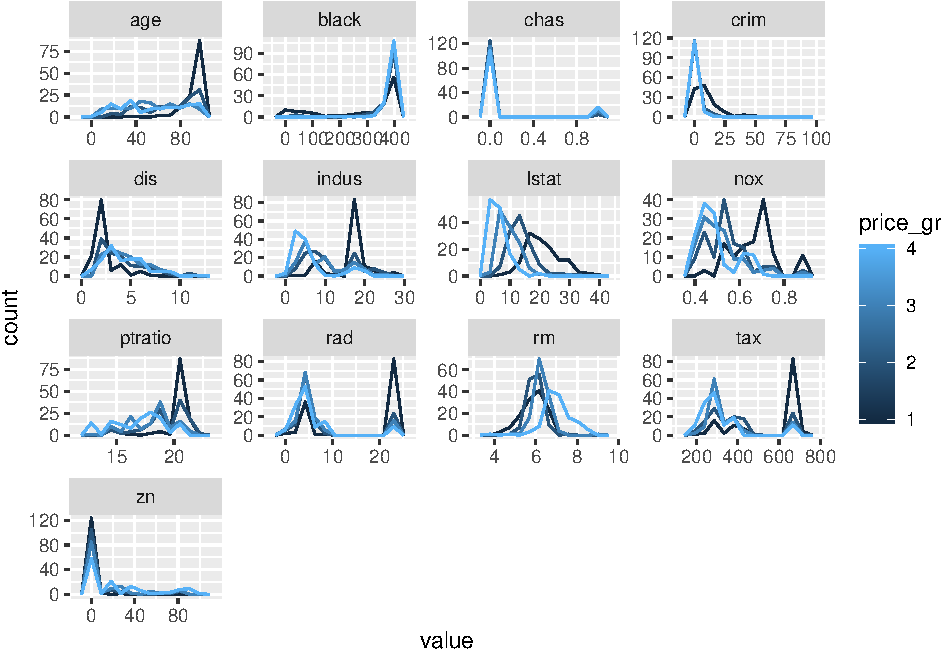
\includegraphics{tidyverse-class_files/figure-latex/cond-hist-1.pdf}

\begin{Shaded}
\begin{Highlighting}[]
\CommentTok{# Click on the expand icon at the top right to make bigger.}
\end{Highlighting}
\end{Shaded}

Appears \texttt{chas} is categorical.

\begin{Shaded}
\begin{Highlighting}[]
\NormalTok{boston <-}\StringTok{ }\NormalTok{boston }\OperatorTok
\StringTok{  }\KeywordTok{mutate}\NormalTok{(}\DataTypeTok{chas =} \KeywordTok{factor}\NormalTok{(chas))}
\end{Highlighting}
\end{Shaded}

Second, scatterplots of median value vs.~all variables.

\begin{Shaded}
\begin{Highlighting}[]
\NormalTok{boston }\OperatorTok
\StringTok{  }\KeywordTok{gather}\NormalTok{(}\StringTok{'key'}\NormalTok{, }\StringTok{'value'}\NormalTok{, }\OperatorTok{-}\KeywordTok{one_of}\NormalTok{(}\KeywordTok{c}\NormalTok{(}\StringTok{"medv"}\NormalTok{, }\StringTok{"chas"}\NormalTok{))) }\OperatorTok\StringTok{ }
\StringTok{  }\KeywordTok{ggplot}\NormalTok{(}\KeywordTok{aes}\NormalTok{(}\DataTypeTok{x =}\NormalTok{ value, }\DataTypeTok{y =}\NormalTok{ medv)) }\OperatorTok{+}
\StringTok{    }\KeywordTok{facet_wrap}\NormalTok{( }\OperatorTok{~}\StringTok{ }\NormalTok{key, }\DataTypeTok{scales =} \StringTok{"free"}\NormalTok{) }\OperatorTok{+}
\StringTok{    }\KeywordTok{geom_point}\NormalTok{(}\KeywordTok{aes}\NormalTok{(}\DataTypeTok{shape =}\NormalTok{ chas), }\DataTypeTok{size =} \FloatTok{0.5}\NormalTok{, }\DataTypeTok{alpha =} \FloatTok{0.25}\NormalTok{) }\OperatorTok{+}
\StringTok{    }\KeywordTok{geom_smooth}\NormalTok{(}\DataTypeTok{lwd =} \FloatTok{0.5}\NormalTok{, }\DataTypeTok{se =} \OtherTok{TRUE}\NormalTok{) }\OperatorTok{+}
\StringTok{  }\KeywordTok{ggsave}\NormalTok{(}\StringTok{'plots/medv-scatter.pdf'}\NormalTok{)}
\end{Highlighting}
\end{Shaded}

\begin{verbatim}
## Saving 6.5 x 4.5 in image
\end{verbatim}

\begin{verbatim}
## `geom_smooth()` using method = 'loess' and formula 'y ~ x'
## `geom_smooth()` using method = 'loess' and formula 'y ~ x'
\end{verbatim}

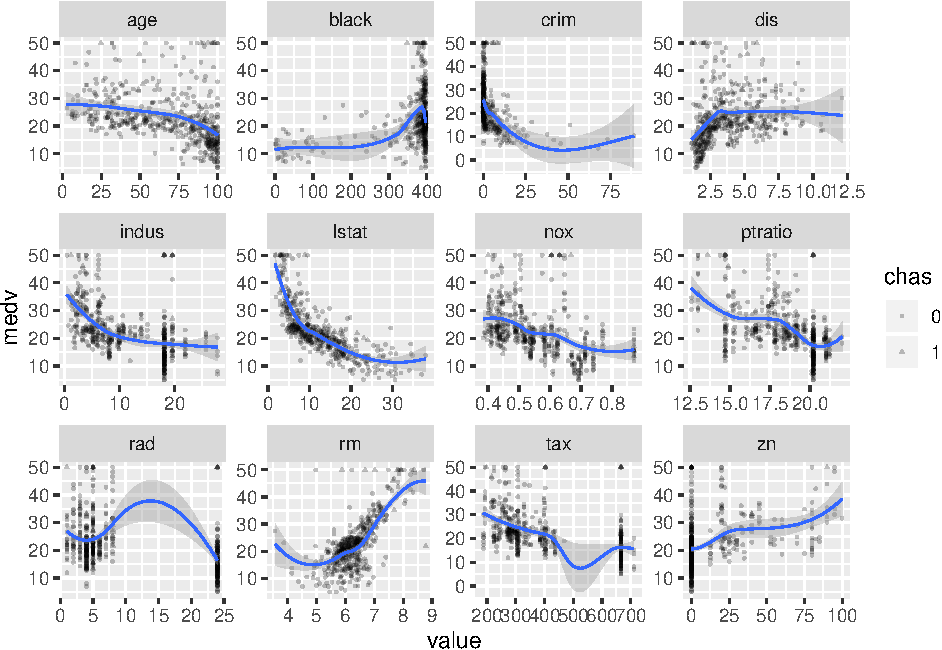
\includegraphics{tidyverse-class_files/figure-latex/medv-scatter-1.pdf}

\begin{Shaded}
\begin{Highlighting}[]
\CommentTok{# Click on the expand icon at the top right to make bigger.}
\end{Highlighting}
\end{Shaded}

There are ggplot jitter options, but none worked for me.

\begin{Shaded}
\begin{Highlighting}[]
\NormalTok{boston }\OperatorTok
\StringTok{  }\KeywordTok{gather}\NormalTok{(}\StringTok{'key'}\NormalTok{, }\StringTok{'value'}\NormalTok{, }\OperatorTok{-}\KeywordTok{one_of}\NormalTok{(}\KeywordTok{c}\NormalTok{(}\StringTok{"medv"}\NormalTok{, }\StringTok{"chas"}\NormalTok{))) }\OperatorTok\StringTok{ }
\StringTok{  }\KeywordTok{ggplot}\NormalTok{(}\KeywordTok{aes}\NormalTok{(}\DataTypeTok{x =}\NormalTok{ value, }\DataTypeTok{y =}\NormalTok{ medv)) }\OperatorTok{+}
\StringTok{    }\KeywordTok{facet_wrap}\NormalTok{( }\OperatorTok{~}\StringTok{ }\NormalTok{key, }\DataTypeTok{scales =} \StringTok{"free"}\NormalTok{) }\OperatorTok{+}
\StringTok{    }\KeywordTok{geom_jitter}\NormalTok{(}\KeywordTok{aes}\NormalTok{(}\DataTypeTok{shape =}\NormalTok{ chas), }\DataTypeTok{size =} \FloatTok{0.5}\NormalTok{, }\DataTypeTok{alpha =} \FloatTok{0.25}\NormalTok{) }\OperatorTok{+}\StringTok{ }
\StringTok{    }\KeywordTok{geom_smooth}\NormalTok{(}\DataTypeTok{lwd =} \FloatTok{0.5}\NormalTok{, }\DataTypeTok{se =} \OtherTok{TRUE}\NormalTok{)}
\end{Highlighting}
\end{Shaded}

\begin{verbatim}
## `geom_smooth()` using method = 'loess' and formula 'y ~ x'
\end{verbatim}

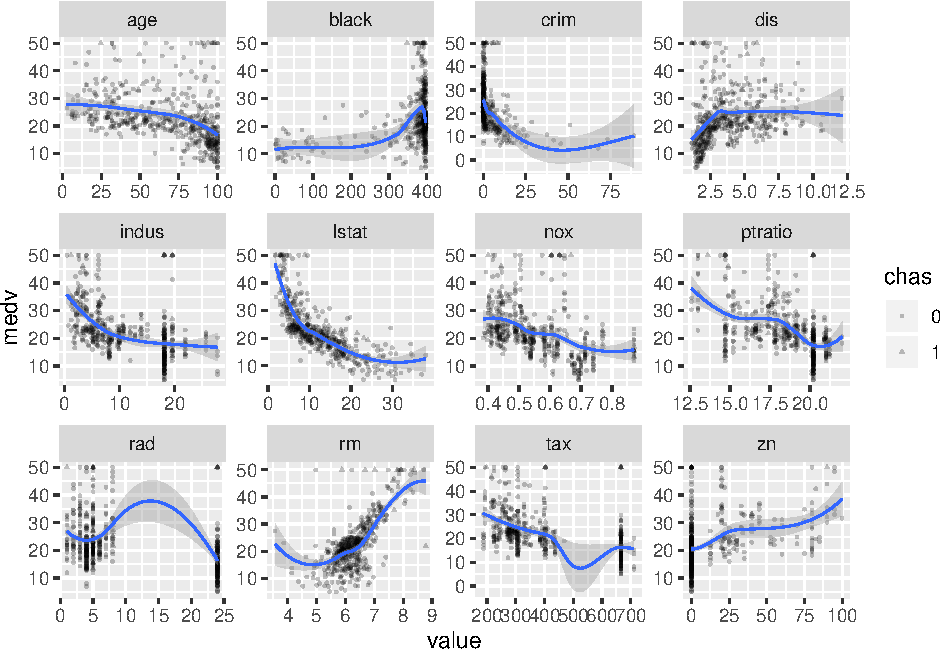
\includegraphics{tidyverse-class_files/figure-latex/medv-jitter-nw-1.pdf}

Tinkering to get a jittered plot.

\begin{Shaded}
\begin{Highlighting}[]
\NormalTok{var_sd <-}\StringTok{ }\NormalTok{boston }\OperatorTok
\StringTok{  }\KeywordTok{gather}\NormalTok{(}\StringTok{'key'}\NormalTok{, }\StringTok{'value'}\NormalTok{, }\OperatorTok{-}\KeywordTok{one_of}\NormalTok{(}\KeywordTok{c}\NormalTok{(}\StringTok{"medv"}\NormalTok{, }\StringTok{"chas"}\NormalTok{))) }\OperatorTok\StringTok{ }
\StringTok{  }\KeywordTok{group_by}\NormalTok{(key) }\OperatorTok\StringTok{ }
\StringTok{  }\KeywordTok{summarize}\NormalTok{(}\DataTypeTok{var_sd =} \KeywordTok{sd}\NormalTok{(value))}
\CommentTok{#var_sd <- boston %>% }
\CommentTok{#  keep(is.numeric) %>% }
\CommentTok{#  summarize_all(sd)}
\NormalTok{boston }\OperatorTok
\StringTok{  }\KeywordTok{gather}\NormalTok{(}\StringTok{'key'}\NormalTok{, }\StringTok{'value'}\NormalTok{, }\OperatorTok{-}\KeywordTok{one_of}\NormalTok{(}\KeywordTok{c}\NormalTok{(}\StringTok{"medv"}\NormalTok{, }\StringTok{"chas"}\NormalTok{))) }\OperatorTok\StringTok{ }
\StringTok{  }\KeywordTok{left_join}\NormalTok{(}\DataTypeTok{y =}\NormalTok{ var_sd, }\DataTypeTok{by =} \StringTok{"key"}\NormalTok{) }\OperatorTok\StringTok{ }
\StringTok{  }\KeywordTok{mutate}\NormalTok{(}\DataTypeTok{jit_val =}\NormalTok{ value }\OperatorTok{+}\StringTok{ }\NormalTok{var_sd }\OperatorTok{*}\StringTok{ }\KeywordTok{runif}\NormalTok{(}\KeywordTok{nrow}\NormalTok{(boston), }\OperatorTok{-}\FloatTok{0.1}\NormalTok{, }\FloatTok{0.1}\NormalTok{)) }\OperatorTok\StringTok{ }
\StringTok{  }\KeywordTok{ggplot}\NormalTok{(}\KeywordTok{aes}\NormalTok{(}\DataTypeTok{x =}\NormalTok{ jit_val, }\DataTypeTok{y =}\NormalTok{ medv)) }\OperatorTok{+}
\StringTok{    }\KeywordTok{facet_wrap}\NormalTok{( }\OperatorTok{~}\StringTok{ }\NormalTok{key, }\DataTypeTok{scales =} \StringTok{"free"}\NormalTok{) }\OperatorTok{+}
\StringTok{    }\KeywordTok{geom_jitter}\NormalTok{(}\KeywordTok{aes}\NormalTok{(}\DataTypeTok{shape =}\NormalTok{ chas), }\DataTypeTok{size =} \FloatTok{0.5}\NormalTok{, }\DataTypeTok{alpha =} \FloatTok{0.25}\NormalTok{) }\OperatorTok{+}
\StringTok{    }\KeywordTok{geom_smooth}\NormalTok{(}\DataTypeTok{lwd =} \FloatTok{0.5}\NormalTok{, }\DataTypeTok{se =} \OtherTok{TRUE}\NormalTok{) }\OperatorTok{+}
\StringTok{  }\KeywordTok{ggsave}\NormalTok{(}\StringTok{'plots/medv-jitter.pdf'}\NormalTok{)}
\end{Highlighting}
\end{Shaded}

\begin{verbatim}
## Saving 6.5 x 4.5 in image
\end{verbatim}

\begin{verbatim}
## `geom_smooth()` using method = 'loess' and formula 'y ~ x'
## `geom_smooth()` using method = 'loess' and formula 'y ~ x'
\end{verbatim}

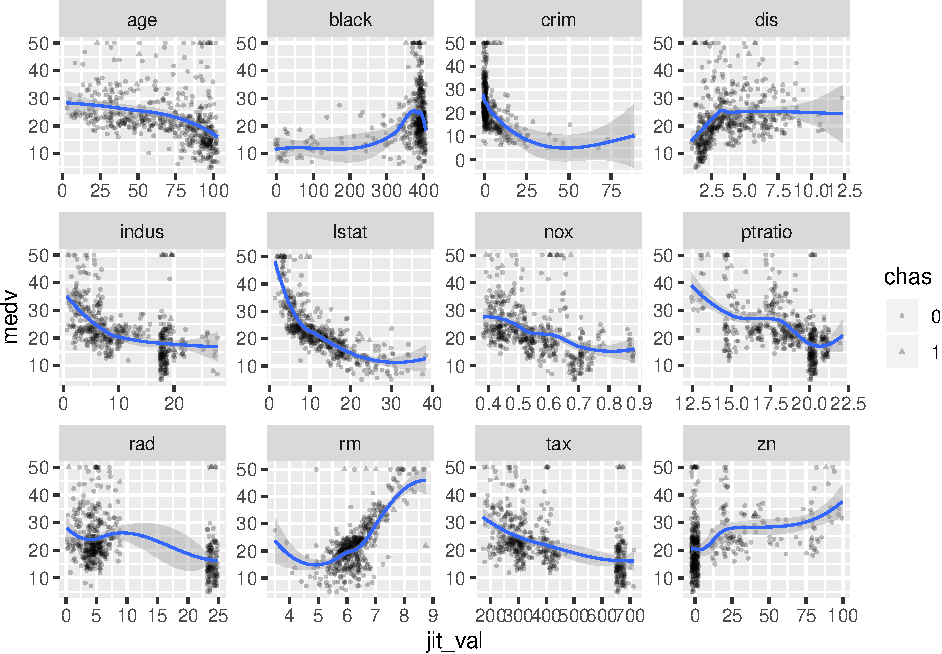
\includegraphics{tidyverse-class_files/figure-latex/medv-jitter-1.pdf}

\begin{Shaded}
\begin{Highlighting}[]
\CommentTok{# Click on the expand icon at the top right to make bigger.}
\end{Highlighting}
\end{Shaded}

Covariance plot of variables.

\begin{Shaded}
\begin{Highlighting}[]
\NormalTok{boston_num <-}\StringTok{ }\NormalTok{boston }\OperatorTok\StringTok{ }
\StringTok{  }\KeywordTok{keep}\NormalTok{(is.numeric) }
\NormalTok{boston_num }\OperatorTok\StringTok{ }
\StringTok{  }\KeywordTok{cor}\NormalTok{() }\OperatorTok\StringTok{ }
\StringTok{  }\KeywordTok{as_tibble}\NormalTok{() }\OperatorTok\StringTok{ }
\StringTok{  }\KeywordTok{mutate}\NormalTok{(}\DataTypeTok{name =} \KeywordTok{colnames}\NormalTok{(boston_num)) }\OperatorTok\StringTok{ }
\StringTok{  }\KeywordTok{gather}\NormalTok{( , , }\OperatorTok{-}\KeywordTok{one_of}\NormalTok{(}\StringTok{"name"}\NormalTok{)) }\OperatorTok\StringTok{ }
\StringTok{  }\KeywordTok{ggplot}\NormalTok{(}\KeywordTok{aes}\NormalTok{(name, key, }\DataTypeTok{fill =}\NormalTok{ value)) }\OperatorTok{+}
\StringTok{    }\KeywordTok{geom_tile}\NormalTok{() }\OperatorTok{+}
\StringTok{    }\KeywordTok{scale_fill_gradient2}\NormalTok{(}\DataTypeTok{low =} \StringTok{"blue"}\NormalTok{, }\DataTypeTok{mid =} \StringTok{"white"}\NormalTok{, }\DataTypeTok{high =} \StringTok{"red"}\NormalTok{,}
                         \DataTypeTok{breaks =} \KeywordTok{seq}\NormalTok{(}\OperatorTok{-}\DecValTok{1}\NormalTok{, }\DecValTok{1}\NormalTok{, , }\DataTypeTok{by =} \FloatTok{0.2}\NormalTok{)) }\OperatorTok{+}
\StringTok{    }\KeywordTok{theme}\NormalTok{(}\DataTypeTok{legend.key.height =} \KeywordTok{unit}\NormalTok{(}\DecValTok{45}\NormalTok{, }\StringTok{"pt"}\NormalTok{))}
\end{Highlighting}
\end{Shaded}

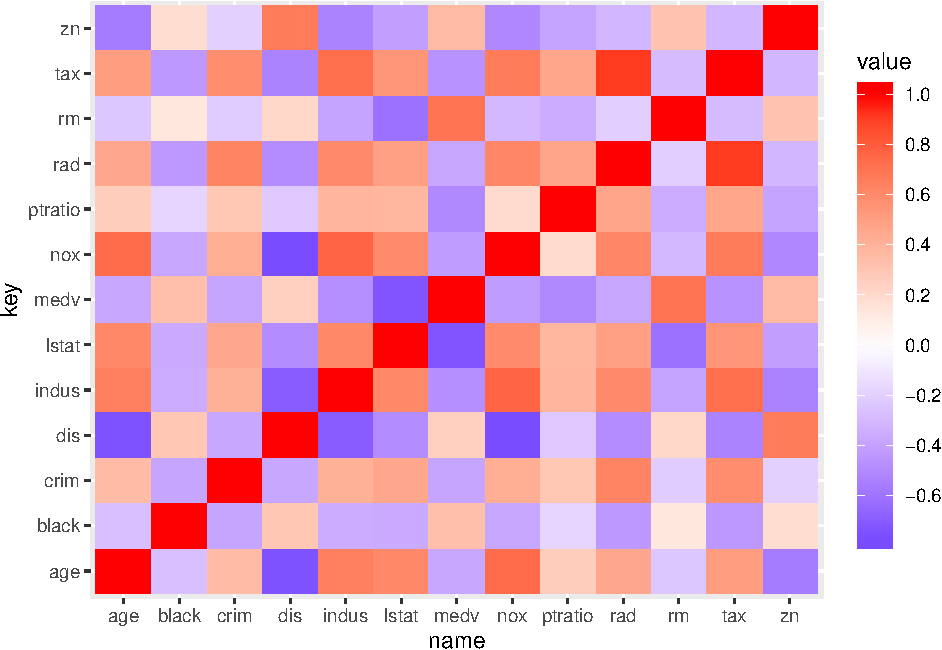
\includegraphics{tidyverse-class_files/figure-latex/cov-plot-1.pdf}

Analyze median value and highway access \texttt{rad}.

\begin{Shaded}
\begin{Highlighting}[]
\NormalTok{boston }\OperatorTok
\StringTok{  }\KeywordTok{ggplot}\NormalTok{(}\KeywordTok{aes}\NormalTok{(rad, medv)) }\OperatorTok{+}
\StringTok{  }\KeywordTok{geom_jitter}\NormalTok{(}\KeywordTok{aes}\NormalTok{(}\DataTypeTok{color =}\NormalTok{ chas), }
              \DataTypeTok{height =} \DecValTok{2}\NormalTok{, }\DataTypeTok{width =} \OtherTok{NULL}\NormalTok{, }
              \DataTypeTok{size =} \DecValTok{1}\NormalTok{, }\DataTypeTok{alpha =} \FloatTok{0.4}\NormalTok{) }\OperatorTok{+}
\StringTok{  }\KeywordTok{geom_smooth}\NormalTok{(}\KeywordTok{aes}\NormalTok{(}\DataTypeTok{color =}\NormalTok{ chas), }\DataTypeTok{lwd =} \DecValTok{1}\NormalTok{)}
\end{Highlighting}
\end{Shaded}

\begin{verbatim}
## `geom_smooth()` using method = 'loess' and formula 'y ~ x'
\end{verbatim}

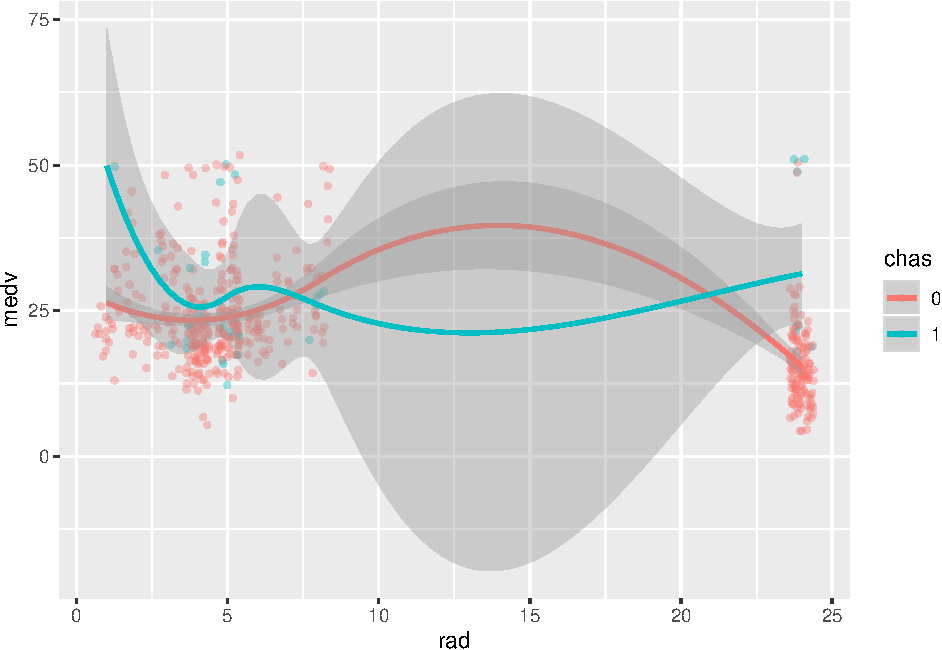
\includegraphics{tidyverse-class_files/figure-latex/medv-rad-1.pdf}

Perhaps \texttt{rad\ =\ 24} is a missing value.

\begin{Shaded}
\begin{Highlighting}[]
\NormalTok{boston }\OperatorTok
\StringTok{  }\KeywordTok{count}\NormalTok{(rad)}
\end{Highlighting}
\end{Shaded}

\begin{verbatim}
## # A tibble: 9 x 2
##     rad     n
##   <int> <int>
## 1     1    20
## 2     2    24
## 3     3    38
## 4     4   110
## 5     5   115
## 6     6    26
## 7     7    17
## 8     8    24
## 9    24   132
\end{verbatim}

\begin{Shaded}
\begin{Highlighting}[]
\NormalTok{boston }\OperatorTok
\StringTok{  }\KeywordTok{gather}\NormalTok{( , , }\OperatorTok{-}\KeywordTok{one_of}\NormalTok{(}\StringTok{"rad"}\NormalTok{)) }\OperatorTok\StringTok{ }
\StringTok{  }\KeywordTok{group_by}\NormalTok{(key, rad) }\OperatorTok
\StringTok{  }\KeywordTok{mutate}\NormalTok{(}\DataTypeTok{value =} \KeywordTok{as.numeric}\NormalTok{(value)) }\OperatorTok\StringTok{  }\CommentTok{# necessary due to factor variable chas}
\StringTok{  }\KeywordTok{summarize}\NormalTok{(}\DataTypeTok{z =} \KeywordTok{round}\NormalTok{(}\KeywordTok{mean}\NormalTok{(value), }\DecValTok{1}\NormalTok{)) }\OperatorTok\StringTok{ }
\StringTok{  }\KeywordTok{spread}\NormalTok{(rad, z)}
\end{Highlighting}
\end{Shaded}

\begin{verbatim}
## Warning: attributes are not identical across measure variables;
## they will be dropped
\end{verbatim}

\begin{verbatim}
## # A tibble: 13 x 10
## # Groups:   key [13]
##    key       `1`   `2`   `3`   `4`   `5`   `6`   `7`   `8`  `24`
##    <chr>   <dbl> <dbl> <dbl> <dbl> <dbl> <dbl> <dbl> <dbl> <dbl>
##  1 age      45    64.8  49.3  60.8  69.2  60.1  40.1  67.3  89.8
##  2 black   389.  386.  392.  383.  369.  387.  388.  385.  288. 
##  3 chas      0     0     0.1   0.1   0.1   0     0     0.2   0.1
##  4 crim      0     0.1   0.1   0.4   0.7   0.2   0.2   0.4  12.8
##  5 dis       6     4.1   5.1   4.4   3.7   4     6.5   4.4   2.1
##  6 indus     5.1   9.6   4.4  10.7   9.8   8.2   5     5.9  18.1
##  7 lstat     7.4  10     9.1  12.2  10.7  12.3   8     8    18.6
##  8 medv     24.4  26.8  27.9  21.4  25.7  21    27.1  30.4  16.4
##  9 nox       0.5   0.5   0.5   0.5   0.6   0.5   0.4   0.5   0.7
## 10 ptratio  17.6  17.3  18.2  19.1  16.5  17.8  18.4  18    20.2
## 11 rm        6.6   6.6   6.5   6.1   6.4   6.1   6.6   7     6  
## 12 tax     291.  261.  246.  336   332.  373.  304.  301.  666  
## 13 zn       39.9  20.4  16.4  14.7  11.1  13    26.7   6.2   0
\end{verbatim}

Or in helpful boxplot format.

\begin{Shaded}
\begin{Highlighting}[]
\NormalTok{boston }\OperatorTok
\StringTok{  }\KeywordTok{keep}\NormalTok{(is.numeric) }\OperatorTok\StringTok{ }
\StringTok{  }\KeywordTok{gather}\NormalTok{( , , }\OperatorTok{-}\KeywordTok{one_of}\NormalTok{(}\StringTok{"rad"}\NormalTok{)) }\OperatorTok\StringTok{ }
\StringTok{  }\KeywordTok{group_by}\NormalTok{(key, rad) }\OperatorTok
\StringTok{  }\KeywordTok{ggplot}\NormalTok{(}\KeywordTok{aes}\NormalTok{(}\DataTypeTok{x =}\NormalTok{ rad, }\DataTypeTok{y =}\NormalTok{ value, }\DataTypeTok{group =}\NormalTok{ rad)) }\OperatorTok{+}\StringTok{ }
\StringTok{    }\KeywordTok{geom_boxplot}\NormalTok{(}\DataTypeTok{outlier.size =} \FloatTok{0.5}\NormalTok{, }\DataTypeTok{varwidth =}\NormalTok{ T) }\OperatorTok{+}
\StringTok{    }\KeywordTok{facet_wrap}\NormalTok{(}\OperatorTok{~}\StringTok{ }\NormalTok{key, }\DataTypeTok{ncol =} \DecValTok{3}\NormalTok{, }\DataTypeTok{scales =} \StringTok{"free"}\NormalTok{) }\OperatorTok{+}
\StringTok{  }\KeywordTok{ggsave}\NormalTok{(}\StringTok{'plots/rad-boxplot.pdf'}\NormalTok{)}
\end{Highlighting}
\end{Shaded}

\begin{verbatim}
## Saving 6.5 x 4.5 in image
\end{verbatim}

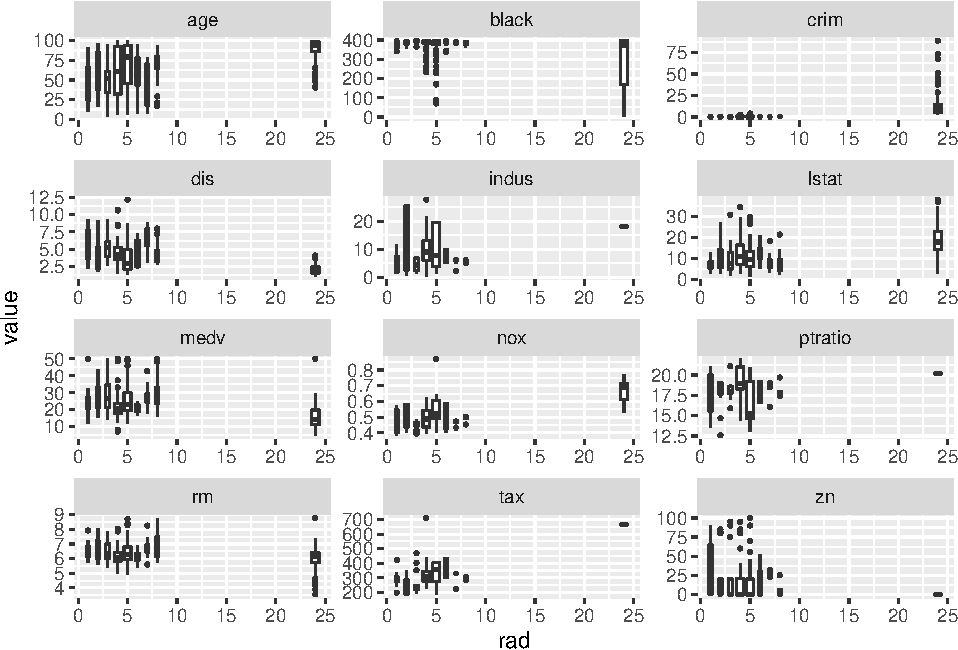
\includegraphics{tidyverse-class_files/figure-latex/boxplot-rad-1.pdf}

Looking at \texttt{lstat} relationships.

\begin{Shaded}
\begin{Highlighting}[]
\NormalTok{boston }\OperatorTok
\StringTok{  }\KeywordTok{keep}\NormalTok{(is.numeric) }\OperatorTok\StringTok{ }
\StringTok{  }\KeywordTok{gather}\NormalTok{( , , }\OperatorTok{-}\KeywordTok{one_of}\NormalTok{(}\StringTok{"lstat"}\NormalTok{)) }\OperatorTok\StringTok{ }
\StringTok{  }\KeywordTok{mutate}\NormalTok{(}\DataTypeTok{lstat_gr =} \KeywordTok{ntile}\NormalTok{(lstat, }\DecValTok{10}\NormalTok{)) }\OperatorTok\StringTok{ }
\StringTok{  }\KeywordTok{group_by}\NormalTok{(key, lstat_gr) }\OperatorTok
\StringTok{  }\KeywordTok{ggplot}\NormalTok{(}\KeywordTok{aes}\NormalTok{(}\DataTypeTok{x =}\NormalTok{ lstat_gr, }\DataTypeTok{y =}\NormalTok{ value, }\DataTypeTok{group =}\NormalTok{ lstat_gr)) }\OperatorTok{+}\StringTok{ }
\StringTok{    }\KeywordTok{geom_violin}\NormalTok{() }\OperatorTok{+}
\StringTok{    }\KeywordTok{facet_wrap}\NormalTok{(}\OperatorTok{~}\StringTok{ }\NormalTok{key, }\DataTypeTok{ncol =} \DecValTok{3}\NormalTok{, }\DataTypeTok{scales =} \StringTok{"free"}\NormalTok{) }\OperatorTok{+}
\StringTok{  }\KeywordTok{ggsave}\NormalTok{(}\StringTok{'plots/lstat-violin.pdf'}\NormalTok{)}
\end{Highlighting}
\end{Shaded}

\begin{verbatim}
## Saving 6.5 x 4.5 in image
\end{verbatim}

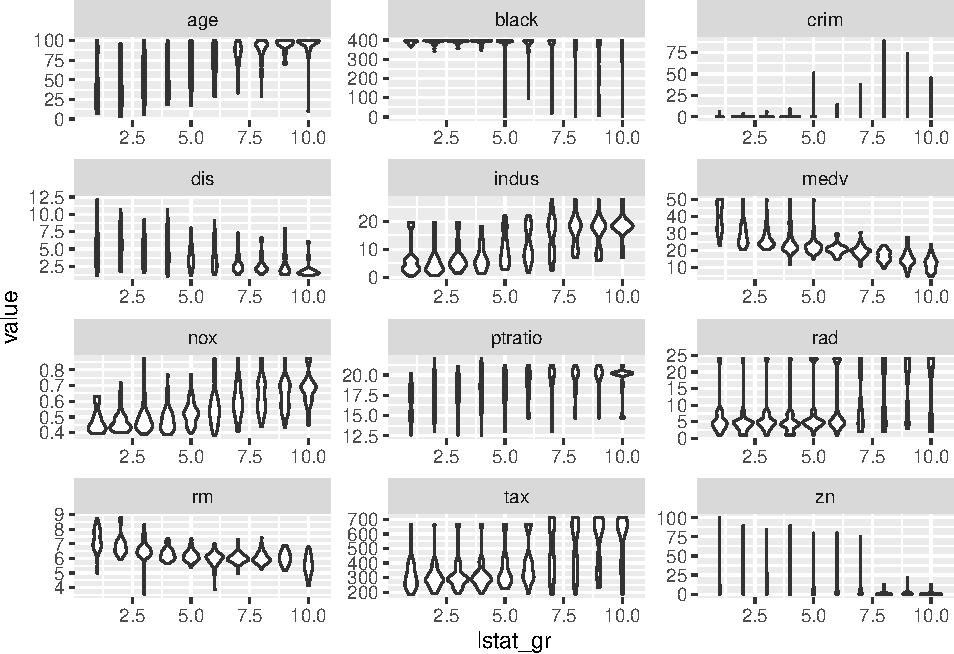
\includegraphics{tidyverse-class_files/figure-latex/violin-lstat-1.pdf}

Jittering works well for single plots.

\begin{Shaded}
\begin{Highlighting}[]
\NormalTok{boston }\OperatorTok
\StringTok{  }\KeywordTok{ggplot}\NormalTok{(}\KeywordTok{aes}\NormalTok{(tax, nox)) }\OperatorTok{+}
\StringTok{    }\KeywordTok{geom_jitter}\NormalTok{(}\KeywordTok{aes}\NormalTok{(}\DataTypeTok{color =}\NormalTok{ medv, }\DataTypeTok{shape =}\NormalTok{ chas), }
                \DataTypeTok{height =} \FloatTok{0.02}\NormalTok{, }\DataTypeTok{width =} \DecValTok{10}\NormalTok{) }\OperatorTok{+}
\StringTok{    }\KeywordTok{scale_color_gradient2}\NormalTok{(}\DataTypeTok{midpoint =} \DecValTok{20}\NormalTok{, }
                          \DataTypeTok{low =} \StringTok{"blue"}\NormalTok{, }\DataTypeTok{mid =} \StringTok{"gray75"}\NormalTok{, }\DataTypeTok{high =} \StringTok{"red"}\NormalTok{) }\OperatorTok{+}
\StringTok{    }\KeywordTok{geom_hline}\NormalTok{(}\DataTypeTok{yintercept =} \FloatTok{0.6}\NormalTok{, }\DataTypeTok{color =} \StringTok{"yellow"}\NormalTok{) }\OperatorTok{+}
\StringTok{    }\KeywordTok{geom_abline}\NormalTok{(}\DataTypeTok{slope =} \FloatTok{0.001}\NormalTok{, }\DataTypeTok{intercept =} \FloatTok{0.1}\NormalTok{, }\DataTypeTok{color =} \StringTok{"blue"}\NormalTok{, }\DataTypeTok{lty =} \StringTok{"93133313"}\NormalTok{)}
\end{Highlighting}
\end{Shaded}

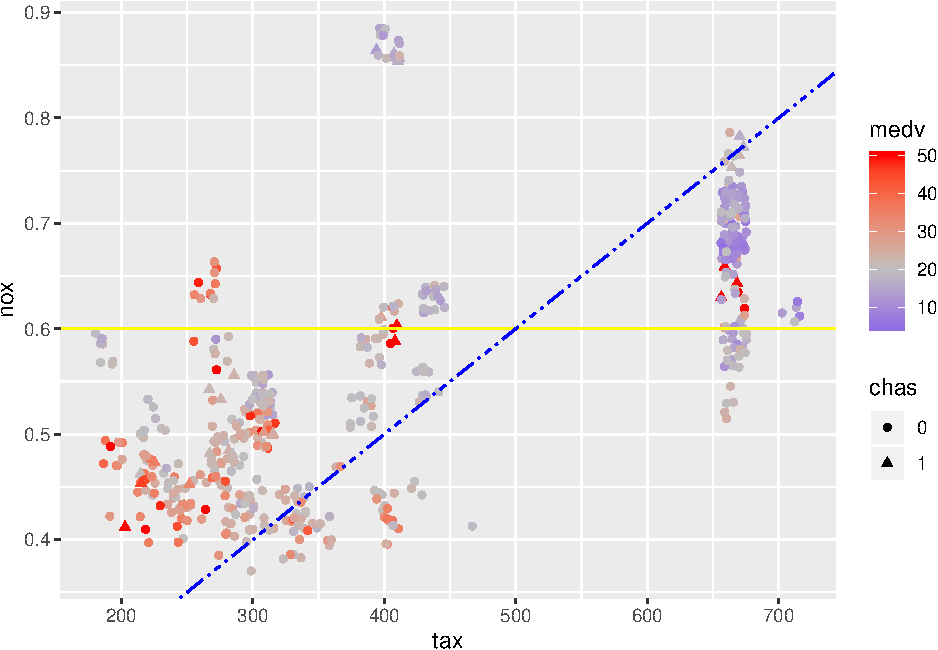
\includegraphics{tidyverse-class_files/figure-latex/tax-nox-1.pdf}

\begin{Shaded}
\begin{Highlighting}[]
  \KeywordTok{ggsave}\NormalTok{(}\StringTok{'plots/tax-nox.pdf'}\NormalTok{)}
\end{Highlighting}
\end{Shaded}

\begin{verbatim}
## Saving 6.5 x 4.5 in image
\end{verbatim}

\section{Many plotting options}\label{many-plotting-options}

Statistics can be added to the plot as an additional layer. Other layers
are coordinates, facets, and scales.

\begin{Shaded}
\begin{Highlighting}[]
\KeywordTok{ggplot}\NormalTok{(}\DataTypeTok{data =}\NormalTok{ boston) }\OperatorTok{+}\StringTok{ }
\StringTok{  }\KeywordTok{geom_point}\NormalTok{(}\DataTypeTok{mapping =} \KeywordTok{aes}\NormalTok{(}\DataTypeTok{x =}\NormalTok{ rm, }\DataTypeTok{y =}\NormalTok{ medv, }\DataTypeTok{color =}\NormalTok{ crim), }\DataTypeTok{alpha=}\FloatTok{0.75}\NormalTok{) }\OperatorTok{+}
\StringTok{  }\KeywordTok{geom_smooth}\NormalTok{(}\DataTypeTok{mapping =} \KeywordTok{aes}\NormalTok{(}\DataTypeTok{x =}\NormalTok{ rm, }\DataTypeTok{y =}\NormalTok{ medv)) }\OperatorTok{+}
\StringTok{  }\KeywordTok{coord_cartesian}\NormalTok{(}\DataTypeTok{xlim =} \KeywordTok{c}\NormalTok{(}\FloatTok{4.5}\NormalTok{, }\FloatTok{7.5}\NormalTok{)) }\OperatorTok{+}
\StringTok{  }\KeywordTok{scale_y_log10}\NormalTok{() }\OperatorTok{+}
\StringTok{  }\KeywordTok{scale_color_gradient}\NormalTok{(}\DataTypeTok{low =} \StringTok{"yellow"}\NormalTok{, }\DataTypeTok{high =} \StringTok{"blue"}\NormalTok{) }\OperatorTok{+}
\StringTok{  }\KeywordTok{labs}\NormalTok{(}\DataTypeTok{x =} \StringTok{"average rooms / house"}\NormalTok{, }\DataTypeTok{y =} \StringTok{"median house price ($K)"}\NormalTok{,}
       \DataTypeTok{title =} \StringTok{"Boston median house prices vs. average house size"}\NormalTok{)}
\end{Highlighting}
\end{Shaded}

\begin{verbatim}
## `geom_smooth()` using method = 'loess' and formula 'y ~ x'
\end{verbatim}

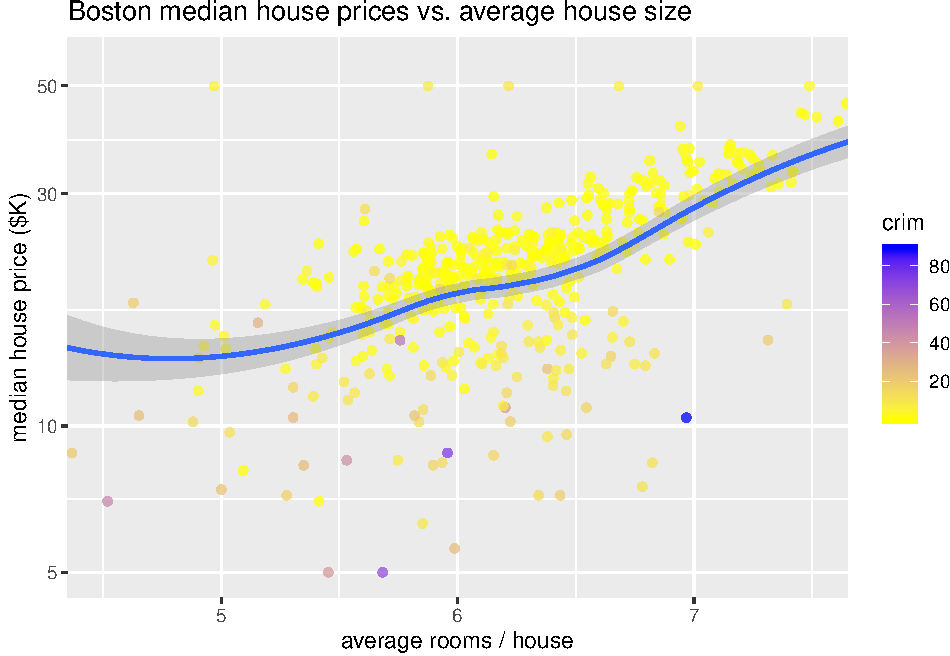
\includegraphics{tidyverse-class_files/figure-latex/price-rooms-2-1.pdf}

Maybe more useful if colored by quantile of \texttt{crim} value.

\begin{Shaded}
\begin{Highlighting}[]
\NormalTok{boston }\OperatorTok\StringTok{ }
\StringTok{  }\KeywordTok{mutate}\NormalTok{(}\DataTypeTok{crim =} \KeywordTok{cume_dist}\NormalTok{(crim)) }\OperatorTok\StringTok{ }
\StringTok{  }\KeywordTok{ggplot}\NormalTok{() }\OperatorTok{+}
\StringTok{    }\KeywordTok{geom_point}\NormalTok{(}\DataTypeTok{mapping =} \KeywordTok{aes}\NormalTok{(}\DataTypeTok{x =}\NormalTok{ rm, }\DataTypeTok{y =}\NormalTok{ medv, }\DataTypeTok{color =}\NormalTok{ crim), }\DataTypeTok{alpha=}\FloatTok{0.75}\NormalTok{) }\OperatorTok{+}
\StringTok{    }\KeywordTok{geom_smooth}\NormalTok{(}\DataTypeTok{mapping =} \KeywordTok{aes}\NormalTok{(}\DataTypeTok{x =}\NormalTok{ rm, }\DataTypeTok{y =}\NormalTok{ medv)) }\OperatorTok{+}
\StringTok{    }\KeywordTok{coord_cartesian}\NormalTok{(}\DataTypeTok{xlim =} \KeywordTok{c}\NormalTok{(}\FloatTok{4.5}\NormalTok{, }\FloatTok{7.5}\NormalTok{)) }\OperatorTok{+}
\StringTok{    }\KeywordTok{scale_y_log10}\NormalTok{() }\OperatorTok{+}
\StringTok{    }\KeywordTok{scale_color_gradient}\NormalTok{(}\DataTypeTok{low =} \StringTok{"yellow"}\NormalTok{, }\DataTypeTok{high =} \StringTok{"blue"}\NormalTok{) }\OperatorTok{+}
\StringTok{    }\KeywordTok{labs}\NormalTok{(}\DataTypeTok{x =} \StringTok{"average rooms / house"}\NormalTok{, }\DataTypeTok{y =} \StringTok{"median house price ($K)"}\NormalTok{,}
       \DataTypeTok{title =} \StringTok{"Boston median house prices, house size, and crime"}\NormalTok{)}
\end{Highlighting}
\end{Shaded}

\begin{verbatim}
## `geom_smooth()` using method = 'loess' and formula 'y ~ x'
\end{verbatim}

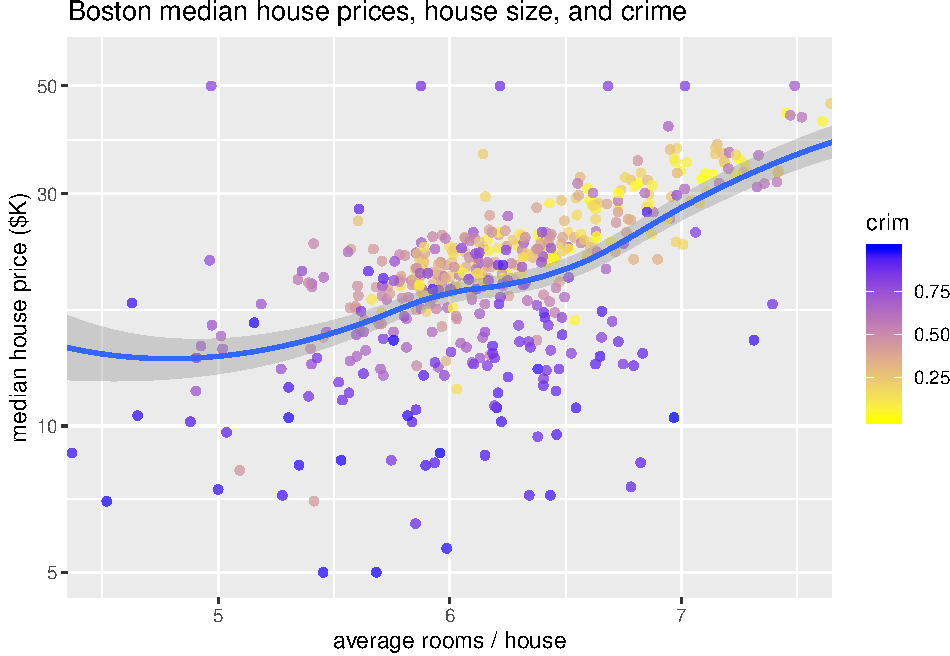
\includegraphics{tidyverse-class_files/figure-latex/price-rooms-3-1.pdf}

Now color by \texttt{rad} but change all 24's to NA's.

\begin{Shaded}
\begin{Highlighting}[]
\NormalTok{boston }\OperatorTok\StringTok{ }
\StringTok{  }\KeywordTok{mutate}\NormalTok{(}\DataTypeTok{rad =} \KeywordTok{ifelse}\NormalTok{(rad }\OperatorTok{==}\StringTok{ }\DecValTok{24}\NormalTok{, }\OtherTok{NA}\NormalTok{, rad)) }\OperatorTok\StringTok{ }
\StringTok{  }\KeywordTok{ggplot}\NormalTok{() }\OperatorTok{+}
\StringTok{    }\KeywordTok{geom_point}\NormalTok{(}\DataTypeTok{mapping =} \KeywordTok{aes}\NormalTok{(}\DataTypeTok{x =}\NormalTok{ rm, }\DataTypeTok{y =}\NormalTok{ medv, }\DataTypeTok{color =}\NormalTok{ rad), }\DataTypeTok{alpha=}\FloatTok{0.75}\NormalTok{) }\OperatorTok{+}
\StringTok{    }\KeywordTok{geom_smooth}\NormalTok{(}\DataTypeTok{mapping =} \KeywordTok{aes}\NormalTok{(}\DataTypeTok{x =}\NormalTok{ rm, }\DataTypeTok{y =}\NormalTok{ medv)) }\OperatorTok{+}
\StringTok{    }\KeywordTok{coord_cartesian}\NormalTok{(}\DataTypeTok{xlim =} \KeywordTok{c}\NormalTok{(}\FloatTok{4.5}\NormalTok{, }\FloatTok{7.5}\NormalTok{)) }\OperatorTok{+}
\StringTok{    }\KeywordTok{scale_y_log10}\NormalTok{() }\OperatorTok{+}
\StringTok{    }\KeywordTok{scale_color_gradient}\NormalTok{(}\DataTypeTok{low =} \StringTok{"yellow"}\NormalTok{, }\DataTypeTok{high =} \StringTok{"red"}\NormalTok{, }\DataTypeTok{na.value =} \StringTok{"black"}\NormalTok{) }\OperatorTok{+}
\StringTok{    }\KeywordTok{labs}\NormalTok{(}\DataTypeTok{x =} \StringTok{"average rooms / house"}\NormalTok{, }\DataTypeTok{y =} \StringTok{"median house price ($K)"}\NormalTok{,}
         \DataTypeTok{title =} \StringTok{"Boston median house prices and access to radial highways"}\NormalTok{)}
\end{Highlighting}
\end{Shaded}

\begin{verbatim}
## `geom_smooth()` using method = 'loess' and formula 'y ~ x'
\end{verbatim}

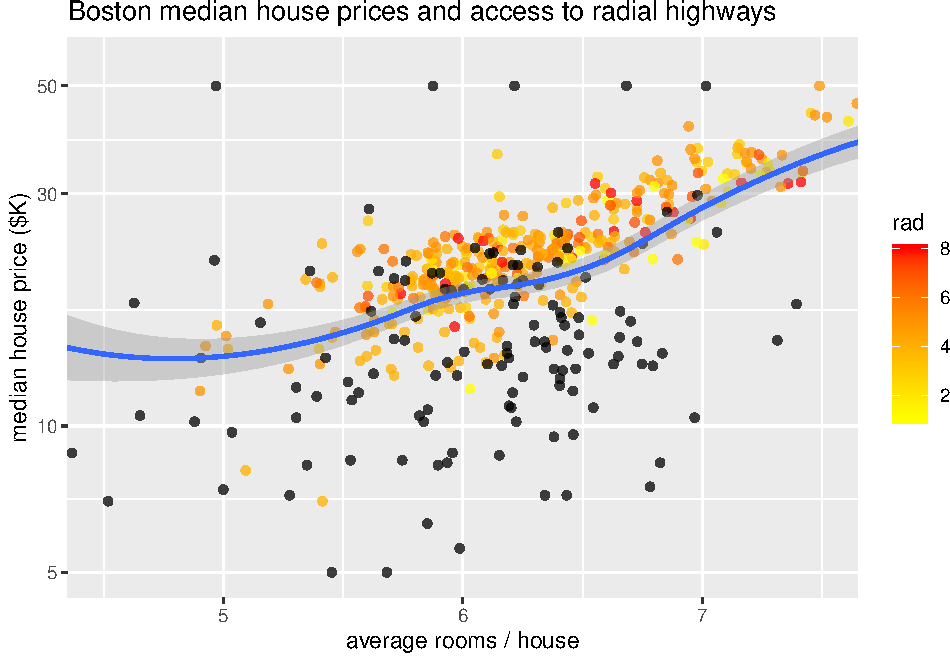
\includegraphics{tidyverse-class_files/figure-latex/price-rad-na-1.pdf}

Maybe excluding newly-NA'ed \texttt{rad} values helps the crime plot.

\begin{Shaded}
\begin{Highlighting}[]
\NormalTok{boston }\OperatorTok\StringTok{ }
\StringTok{  }\KeywordTok{mutate}\NormalTok{(}\DataTypeTok{rad =} \KeywordTok{ifelse}\NormalTok{(rad }\OperatorTok{==}\StringTok{ }\DecValTok{24}\NormalTok{, }\OtherTok{NA}\NormalTok{, rad)) }\OperatorTok\StringTok{ }
\StringTok{  }\KeywordTok{mutate}\NormalTok{(}\DataTypeTok{crim =} \KeywordTok{cume_dist}\NormalTok{(crim)) }\OperatorTok\StringTok{ }
\StringTok{  }\KeywordTok{filter}\NormalTok{(}\OperatorTok{!}\KeywordTok{is.na}\NormalTok{(rad)) }\OperatorTok\StringTok{ }
\StringTok{  }\KeywordTok{ggplot}\NormalTok{() }\OperatorTok{+}
\StringTok{    }\KeywordTok{geom_point}\NormalTok{(}\DataTypeTok{mapping =} \KeywordTok{aes}\NormalTok{(}\DataTypeTok{x =}\NormalTok{ rm, }\DataTypeTok{y =}\NormalTok{ medv, }\DataTypeTok{color =}\NormalTok{ crim), }\DataTypeTok{size =} \DecValTok{1}\NormalTok{) }\OperatorTok{+}
\StringTok{    }\KeywordTok{geom_smooth}\NormalTok{(}\DataTypeTok{mapping =} \KeywordTok{aes}\NormalTok{(}\DataTypeTok{x =}\NormalTok{ rm, }\DataTypeTok{y =}\NormalTok{ medv), }\DataTypeTok{lwd =} \FloatTok{0.5}\NormalTok{) }\OperatorTok{+}
\StringTok{    }\KeywordTok{scale_y_log10}\NormalTok{() }\OperatorTok{+}
\StringTok{    }\KeywordTok{scale_color_gradient}\NormalTok{(}\DataTypeTok{low =} \StringTok{"yellow"}\NormalTok{, }\DataTypeTok{high =} \StringTok{"blue"}\NormalTok{) }\OperatorTok{+}
\StringTok{    }\KeywordTok{labs}\NormalTok{(}\DataTypeTok{x =} \StringTok{"average rooms / house"}\NormalTok{, }\DataTypeTok{y =} \StringTok{"median house price ($K)"}\NormalTok{,}
       \DataTypeTok{title =} \StringTok{"Boston median house prices, house size, and crime"}\NormalTok{)}
\end{Highlighting}
\end{Shaded}

\begin{verbatim}
## `geom_smooth()` using method = 'loess' and formula 'y ~ x'
\end{verbatim}

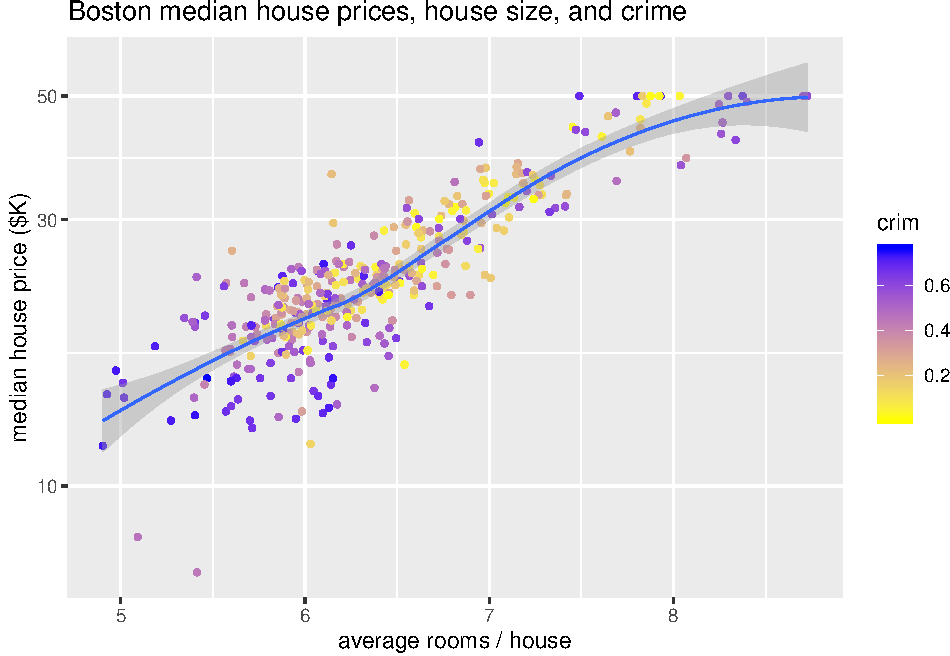
\includegraphics{tidyverse-class_files/figure-latex/price-rooms-4-1.pdf}

A grid of \texttt{nox} vs. \texttt{dis} plots according to \texttt{chas}
(rows) and binned level (ntile) of \texttt{rad}.

\begin{Shaded}
\begin{Highlighting}[]
\NormalTok{boston }\OperatorTok
\StringTok{  }\KeywordTok{mutate}\NormalTok{(}\DataTypeTok{rad =} \KeywordTok{ifelse}\NormalTok{(rad }\OperatorTok{==}\StringTok{ }\DecValTok{24}\NormalTok{, }\OtherTok{NA}\NormalTok{, rad)) }\OperatorTok\StringTok{ }
\StringTok{  }\KeywordTok{filter}\NormalTok{(}\OperatorTok{!}\KeywordTok{is.na}\NormalTok{(rad)) }\OperatorTok\StringTok{ }
\StringTok{  }\KeywordTok{ggplot}\NormalTok{(}\KeywordTok{aes}\NormalTok{(nox, dis, }\DataTypeTok{color =}\NormalTok{ medv)) }\OperatorTok{+}
\StringTok{    }\KeywordTok{geom_jitter}\NormalTok{() }\OperatorTok{+}
\StringTok{    }\KeywordTok{facet_grid}\NormalTok{(chas }\OperatorTok{~}\StringTok{ }\KeywordTok{ntile}\NormalTok{(rad, }\DecValTok{3}\NormalTok{)) }\OperatorTok{+}
\StringTok{    }\KeywordTok{geom_smooth}\NormalTok{()}
\end{Highlighting}
\end{Shaded}

\begin{verbatim}
## `geom_smooth()` using method = 'loess' and formula 'y ~ x'
\end{verbatim}

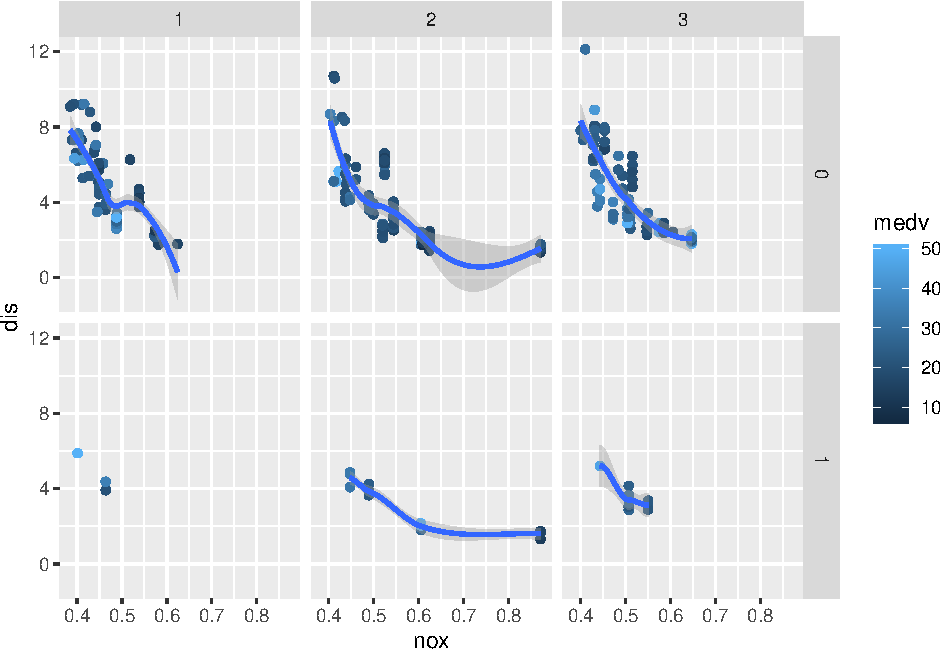
\includegraphics{tidyverse-class_files/figure-latex/facet-grid-1.pdf}

Multiplots available with \texttt{gridExtra}, used by ggplot2.

\begin{Shaded}
\begin{Highlighting}[]
\KeywordTok{require}\NormalTok{(gridExtra)}
\NormalTok{p1 <-}\StringTok{ }\KeywordTok{ggplot}\NormalTok{(boston) }\OperatorTok{+}
\StringTok{  }\KeywordTok{geom_point}\NormalTok{(}\KeywordTok{aes}\NormalTok{(nox, medv, }\DataTypeTok{shape =}\NormalTok{ chas, }\DataTypeTok{alpha =} \KeywordTok{cume_dist}\NormalTok{(lstat)), }
             \DataTypeTok{color =} \StringTok{'red'}\NormalTok{, }\DataTypeTok{size =} \DecValTok{2}\NormalTok{) }\OperatorTok{+}
\StringTok{  }\KeywordTok{labs}\NormalTok{(}\DataTypeTok{title =} \StringTok{'using aes(alpha, shape)'}\NormalTok{)}
\NormalTok{p2 <-}\StringTok{ }\NormalTok{boston }\OperatorTok
\StringTok{  }\KeywordTok{mutate}\NormalTok{(}\DataTypeTok{lstat_gr =} \KeywordTok{ntile}\NormalTok{(lstat, }\DecValTok{3}\NormalTok{)) }\OperatorTok\StringTok{ }
\StringTok{  }\KeywordTok{ggplot}\NormalTok{(}\KeywordTok{aes}\NormalTok{(tax, medv, }\DataTypeTok{color =}\NormalTok{ lstat_gr, }\DataTypeTok{size =}\NormalTok{ nox)) }\OperatorTok{+}\StringTok{ }
\StringTok{  }\KeywordTok{geom_point}\NormalTok{(}\DataTypeTok{shape =} \DecValTok{16}\NormalTok{, }\DataTypeTok{alpha =} \FloatTok{0.75}\NormalTok{) }\OperatorTok{+}
\StringTok{  }\KeywordTok{geom_smooth}\NormalTok{(}\KeywordTok{aes}\NormalTok{(}\DataTypeTok{group =}\NormalTok{ lstat_gr), }\DataTypeTok{lwd =} \FloatTok{0.8}\NormalTok{) }\OperatorTok{+}
\StringTok{  }\KeywordTok{labs}\NormalTok{(}\DataTypeTok{title =} \StringTok{'using aes(group, size)'}\NormalTok{)}
\NormalTok{p1}
\end{Highlighting}
\end{Shaded}

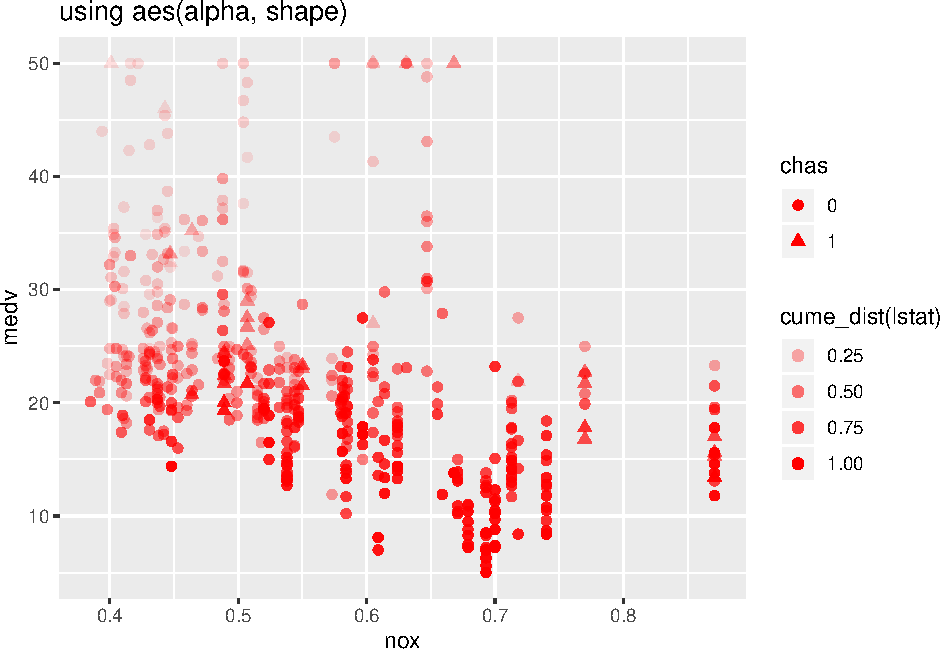
\includegraphics{tidyverse-class_files/figure-latex/multiple-plots-1.pdf}

\begin{Shaded}
\begin{Highlighting}[]
\NormalTok{p2}
\end{Highlighting}
\end{Shaded}

\begin{verbatim}
## `geom_smooth()` using method = 'loess' and formula 'y ~ x'
\end{verbatim}

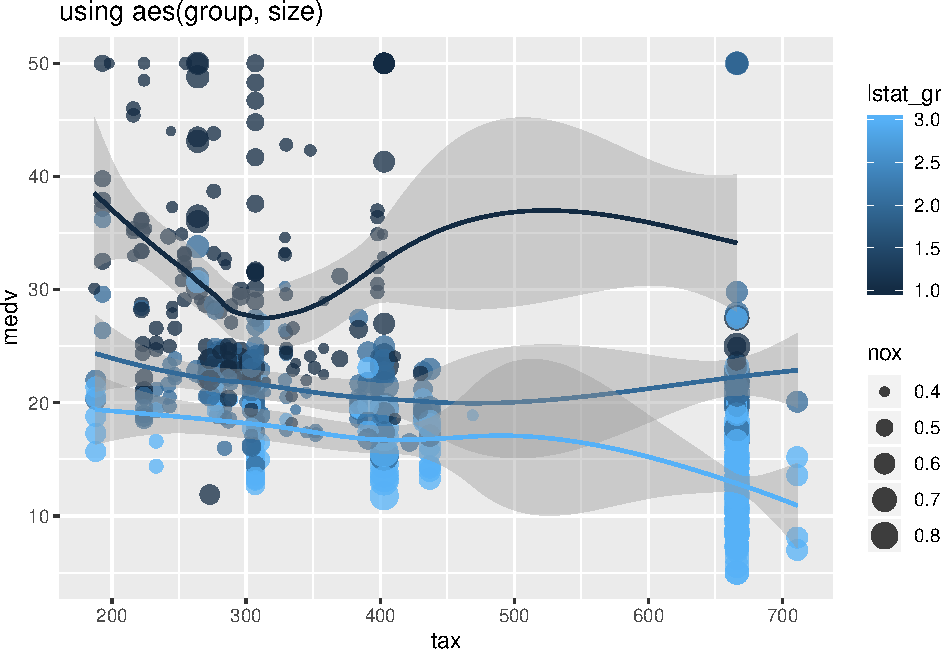
\includegraphics{tidyverse-class_files/figure-latex/multiple-plots-2.pdf}

\begin{Shaded}
\begin{Highlighting}[]
\KeywordTok{ggsave}\NormalTok{(}\StringTok{'plots/two-plot.pdf'}\NormalTok{, }\KeywordTok{arrangeGrob}\NormalTok{(p1, p2))}
\end{Highlighting}
\end{Shaded}

\begin{verbatim}
## Saving 6.5 x 4.5 in image
## `geom_smooth()` using method = 'loess' and formula 'y ~ x'
\end{verbatim}

\chapter{dplyr and tidyr}\label{ch:dplyr}

\begin{Shaded}
\begin{Highlighting}[]
\KeywordTok{library}\NormalTok{(tidyverse)}
\KeywordTok{library}\NormalTok{(gridExtra)}
\NormalTok{batting <-}\StringTok{ }\KeywordTok{as_tibble}\NormalTok{(Lahman}\OperatorTok{::}\NormalTok{Batting)}
\NormalTok{fielding <-}\StringTok{ }\KeywordTok{as_tibble}\NormalTok{(Lahman}\OperatorTok{::}\NormalTok{Fielding)}
\end{Highlighting}
\end{Shaded}

\section{Hoofin' it with dplyr}\label{hoofin-it-with-dplyr}

Condense batting stats into player career totals, keep only those
\textgreater{}= 500 games.

\begin{Shaded}
\begin{Highlighting}[]
\NormalTok{is_col <-}\StringTok{ }\KeywordTok{names}\NormalTok{(batting)[}\KeywordTok{c}\NormalTok{(}\DecValTok{1}\NormalTok{, }\DecValTok{2}\NormalTok{, }\DecValTok{4}\NormalTok{, }\DecValTok{6}\OperatorTok{:}\DecValTok{17}\NormalTok{)]}
\NormalTok{is_num <-}\StringTok{ }\KeywordTok{names}\NormalTok{(batting)[}\KeywordTok{sapply}\NormalTok{(batting, is.numeric)]}
\NormalTok{gt_}\DecValTok{500}\NormalTok{ <-}\StringTok{ }\NormalTok{batting }\OperatorTok
\StringTok{  }\KeywordTok{select}\NormalTok{(is_col) }\OperatorTok
\StringTok{  }\KeywordTok{select}\NormalTok{(}\OperatorTok{-}\NormalTok{teamID) }\OperatorTok\StringTok{ }
\StringTok{  }\KeywordTok{drop_na}\NormalTok{() }\OperatorTok
\StringTok{  }\KeywordTok{group_by}\NormalTok{(playerID) }\OperatorTok\StringTok{ }
\StringTok{  }\KeywordTok{summarize_at}\NormalTok{(is_col[}\OperatorTok{-}\NormalTok{(}\DecValTok{1}\OperatorTok{:}\DecValTok{3}\NormalTok{)], sum, }\DataTypeTok{na.rm =}\NormalTok{ T) }\OperatorTok\StringTok{ }
\StringTok{  }\KeywordTok{filter}\NormalTok{(G }\OperatorTok{>=}\StringTok{ }\DecValTok{500}\NormalTok{)}
\end{Highlighting}
\end{Shaded}

All Ha\textasciitilde{} Green\textasciitilde{} statistics:

\begin{Shaded}
\begin{Highlighting}[]
\NormalTok{batting }\OperatorTok
\StringTok{  }\KeywordTok{filter}\NormalTok{(}\KeywordTok{str_detect}\NormalTok{(playerID, }\StringTok{"greenha"}\NormalTok{))}
\end{Highlighting}
\end{Shaded}

\begin{verbatim}
## # A tibble: 14 x 22
##    playerID yearID stint teamID lgID      G    AB     R     H   X2B   X3B
##    <chr>     <int> <int> <fct>  <fct> <int> <int> <int> <int> <int> <int>
##  1 greenha~   1930     1 DET    AL        1     1     0     0     0     0
##  2 greenha~   1933     1 DET    AL      117   449    59   135    33     3
##  3 greenha~   1934     1 DET    AL      153   593   118   201    63     7
##  4 greenha~   1935     1 DET    AL      152   619   121   203    46    16
##  5 greenha~   1935     1 BRO    NL        2     0     0     0     0     0
##  6 greenha~   1936     1 DET    AL       12    46    10    16     6     2
##  7 greenha~   1937     1 DET    AL      154   594   137   200    49    14
##  8 greenha~   1938     1 DET    AL      155   556   144   175    23     4
##  9 greenha~   1939     1 DET    AL      138   500   112   156    42     7
## 10 greenha~   1940     1 DET    AL      148   573   129   195    50     8
## 11 greenha~   1941     1 DET    AL       19    67    12    18     5     1
## 12 greenha~   1945     1 DET    AL       78   270    47    84    20     2
## 13 greenha~   1946     1 DET    AL      142   523    91   145    29     5
## 14 greenha~   1947     1 PIT    NL      125   402    71   100    13     2
## # ... with 11 more variables: HR <int>, RBI <int>, SB <int>, CS <int>,
## #   BB <int>, SO <int>, IBB <int>, HBP <int>, SH <int>, SF <int>,
## #   GIDP <int>
\end{verbatim}

Positions by game.

\begin{Shaded}
\begin{Highlighting}[]
\NormalTok{fielding }\OperatorTok\StringTok{ }
\StringTok{  }\KeywordTok{group_by}\NormalTok{(POS) }\OperatorTok\StringTok{ }
\StringTok{  }\KeywordTok{count}\NormalTok{(}\DataTypeTok{wt =}\NormalTok{ G)}
\end{Highlighting}
\end{Shaded}

\begin{verbatim}
## # A tibble: 7 x 2
## # Groups:   POS [7]
##   POS         n
##   <chr>   <int>
## 1 1B     482698
## 2 2B     480968
## 3 3B     482320
## 4 C      497547
## 5 OF    1451301
## 6 P     1106574
## 7 SS     479045
\end{verbatim}

Attach a column denoting their main fielding position.

\begin{Shaded}
\begin{Highlighting}[]
\NormalTok{is_field =}\StringTok{ }\KeywordTok{names}\NormalTok{(fielding)[}\KeywordTok{c}\NormalTok{(}\DecValTok{1}\NormalTok{, }\DecValTok{6}\NormalTok{, }\DecValTok{7}\NormalTok{, }\DecValTok{9}\NormalTok{, }\DecValTok{10}\NormalTok{, }\DecValTok{11}\NormalTok{, }\DecValTok{12}\NormalTok{, }\DecValTok{13}\NormalTok{)]}
\NormalTok{fielding }\OperatorTok
\StringTok{  }\KeywordTok{select}\NormalTok{(is_field) }\OperatorTok\StringTok{ }
\StringTok{  }\KeywordTok{map}\NormalTok{(}\OperatorTok{~}\StringTok{ }\KeywordTok{sum}\NormalTok{(}\KeywordTok{is.na}\NormalTok{(.)))}
\end{Highlighting}
\end{Shaded}

\begin{verbatim}
## $playerID
## [1] 0
## 
## $POS
## [1] 0
## 
## $G
## [1] 0
## 
## $InnOuts
## [1] 29929
## 
## $PO
## [1] 0
## 
## $A
## [1] 0
## 
## $E
## [1] 1
## 
## $DP
## [1] 0
\end{verbatim}

Removing InnOuts is a good idea, too many missing.

\begin{Shaded}
\begin{Highlighting}[]
\NormalTok{is_field =}\StringTok{ }\KeywordTok{names}\NormalTok{(fielding)[}\KeywordTok{c}\NormalTok{(}\DecValTok{1}\NormalTok{, }\DecValTok{6}\NormalTok{, }\DecValTok{7}\NormalTok{, }\DecValTok{10}\NormalTok{, }\DecValTok{11}\NormalTok{, }\DecValTok{12}\NormalTok{, }\DecValTok{13}\NormalTok{)]}
\NormalTok{pos_tot <-}\StringTok{ }\NormalTok{fielding }\OperatorTok
\StringTok{  }\KeywordTok{select}\NormalTok{(is_field) }\OperatorTok\StringTok{ }
\StringTok{  }\KeywordTok{drop_na}\NormalTok{() }\OperatorTok\StringTok{ }
\StringTok{  }\KeywordTok{group_by}\NormalTok{(playerID, POS) }\OperatorTok
\StringTok{  }\KeywordTok{summarize_all}\NormalTok{(sum) }\OperatorTok
\StringTok{  }\KeywordTok{ungroup}\NormalTok{() }\OperatorTok\StringTok{ }
\StringTok{  }\KeywordTok{filter}\NormalTok{(G }\OperatorTok{>=}\StringTok{ }\DecValTok{100}\NormalTok{) }\OperatorTok\StringTok{ }
\StringTok{  }\KeywordTok{arrange}\NormalTok{(playerID, }\KeywordTok{desc}\NormalTok{(G)) }\OperatorTok
\StringTok{  }\KeywordTok{group_by}\NormalTok{(playerID) }\OperatorTok\StringTok{ }
\StringTok{  }\KeywordTok{mutate}\NormalTok{(}\DataTypeTok{pos1 =} \KeywordTok{first}\NormalTok{(POS)) }\OperatorTok\StringTok{ }
\StringTok{  }\KeywordTok{filter}\NormalTok{(POS }\OperatorTok{==}\StringTok{ }\NormalTok{pos1) }\OperatorTok\StringTok{ }
\StringTok{  }\KeywordTok{select}\NormalTok{(}\OperatorTok{-}\NormalTok{pos1)}
\end{Highlighting}
\end{Shaded}

\section{tidyr and relational data}\label{tidyr-and-relational-data}

Add fielding info to batting tibble.

\begin{Shaded}
\begin{Highlighting}[]
\NormalTok{(batpos <-}\StringTok{ }\NormalTok{gt_}\DecValTok{500} \OperatorTok\StringTok{ }
\StringTok{   }\KeywordTok{left_join}\NormalTok{(pos_tot, }\DataTypeTok{by =} \StringTok{"playerID"}\NormalTok{))}
\end{Highlighting}
\end{Shaded}

\begin{verbatim}
## # A tibble: 2,667 x 19
##    playerID   G.x    AB     R     H   X2B   X3B    HR   RBI    SB    CS
##    <chr>    <int> <int> <int> <int> <int> <int> <int> <int> <int> <int>
##  1 aaronha~  3298 12364  2174  3771   624    98   755  2297   240    73
##  2 abbotku~   702  2044   273   523   109    23    62   242    22    11
##  3 abernte~   681   181    12    25     3     0     0     9     0     0
##  4 abramca~   521  1543   246   422    62    19    32   134    11    18
##  5 abreubo~  2425  8480  1453  2470   574    59   288  1363   400   128
##  6 abreujo~   742  2913   398   858   180    13   146   488     8     3
##  7 ackledu~   635  2125   261   512    94    18    46   216    31    12
##  8 adairje~  1165  4019   378  1022   163    19    57   366    29    29
##  9 adamsbo~   797  2604   395   701   107    31    25   188    25    30
## 10 adamsgl~   661  1617   152   452    79     5    34   225     6    10
## # ... with 2,657 more rows, and 8 more variables: BB <int>, SO <int>,
## #   POS <chr>, G.y <int>, PO <int>, A <int>, E <int>, DP <int>
\end{verbatim}

Counts of positions.

\begin{Shaded}
\begin{Highlighting}[]
\NormalTok{batpos }\OperatorTok\StringTok{ }
\StringTok{  }\KeywordTok{group_by}\NormalTok{(POS) }\OperatorTok\StringTok{ }
\StringTok{  }\KeywordTok{count}\NormalTok{()}
\end{Highlighting}
\end{Shaded}

\begin{verbatim}
## # A tibble: 8 x 2
## # Groups:   POS [8]
##   POS       n
##   <chr> <int>
## 1 <NA>      2
## 2 1B      254
## 3 2B      277
## 4 3B      270
## 5 C       300
## 6 OF      890
## 7 P       378
## 8 SS      296
\end{verbatim}

NAs are likely DHs.

\begin{Shaded}
\begin{Highlighting}[]
\NormalTok{pos_nas <-}\StringTok{ }\NormalTok{batpos }\OperatorTok\StringTok{ }
\StringTok{  }\KeywordTok{filter}\NormalTok{(}\KeywordTok{is.na}\NormalTok{(POS))}
\NormalTok{batting }\OperatorTok\StringTok{ }
\StringTok{  }\KeywordTok{inner_join}\NormalTok{(pos_nas, }\DataTypeTok{by =} \StringTok{"playerID"}\NormalTok{)}
\end{Highlighting}
\end{Shaded}

\begin{verbatim}
## # A tibble: 26 x 40
##    playerID yearID stint teamID lgID      G  AB.x   R.x   H.x X2B.x X3B.x
##    <chr>     <int> <int> <fct>  <fct> <int> <int> <int> <int> <int> <int>
##  1 moraljo~   1973     1 OAK    AL        6    14     0     4     1     0
##  2 moraljo~   1973     2 MON    NL        5     5     0     2     0     0
##  3 moraljo~   1974     1 MON    NL       25    26     3     7     4     0
##  4 moraljo~   1975     1 MON    NL       93   163    18    49     6     1
##  5 moraljo~   1976     1 MON    NL      104   158    12    50    11     0
##  6 moraljo~   1977     1 MON    NL       65    74     3    15     4     1
##  7 moraljo~   1978     1 MIN    AL      101   242    22    76    13     1
##  8 moraljo~   1979     1 MIN    AL       92   191    21    51     5     1
##  9 moraljo~   1980     1 MIN    AL       97   241    36    73    17     2
## 10 moraljo~   1981     1 BAL    AL       38    86     6    21     3     0
## # ... with 16 more rows, and 29 more variables: HR.x <int>, RBI.x <int>,
## #   SB.x <int>, CS.x <int>, BB.x <int>, SO.x <int>, IBB <int>, HBP <int>,
## #   SH <int>, SF <int>, GIDP <int>, G.x <int>, AB.y <int>, R.y <int>,
## #   H.y <int>, X2B.y <int>, X3B.y <int>, HR.y <int>, RBI.y <int>,
## #   SB.y <int>, CS.y <int>, BB.y <int>, SO.y <int>, POS <chr>, G.y <int>,
## #   PO <int>, A <int>, E <int>, DP <int>
\end{verbatim}

Drop these two DHs.

\begin{Shaded}
\begin{Highlighting}[]
\NormalTok{batpos <-}\StringTok{ }\NormalTok{batpos }\OperatorTok\StringTok{ }
\StringTok{  }\KeywordTok{drop_na}\NormalTok{()}
\end{Highlighting}
\end{Shaded}

Now we could explore many aspects of hitting stats vs.~position, and see
what position players were better fielders or better hitters, or if
neither we can see if they played for the Expos.

\begin{Shaded}
\begin{Highlighting}[]
\NormalTok{batpos }\OperatorTok\StringTok{ }
\StringTok{  }\KeywordTok{filter}\NormalTok{(POS }\OperatorTok{==}\StringTok{ "SS"}\NormalTok{) }\OperatorTok\StringTok{ }
\StringTok{  }\KeywordTok{mutate}\NormalTok{(}\DataTypeTok{BA =}\NormalTok{ H }\OperatorTok{/}\StringTok{ }\NormalTok{AB) }\OperatorTok\StringTok{  }\CommentTok{# batting average, hits / at bats}
\StringTok{  }\KeywordTok{mutate}\NormalTok{(}\DataTypeTok{Err =}\NormalTok{ E }\OperatorTok{/}\StringTok{ }\NormalTok{(PO }\OperatorTok{+}\StringTok{ }\NormalTok{A)) }\OperatorTok\StringTok{   }\CommentTok{# error rate, errors / (put outs + assists)}
\StringTok{  }\KeywordTok{mutate}\NormalTok{(}\DataTypeTok{HRR =}\NormalTok{ HR }\OperatorTok{/}\StringTok{ }\NormalTok{AB) }\OperatorTok\StringTok{  }\CommentTok{# home run rate, home runs / at bats}
\StringTok{  }\KeywordTok{ggplot}\NormalTok{(}\KeywordTok{aes}\NormalTok{(Err, BA)) }\OperatorTok{+}
\StringTok{    }\KeywordTok{geom_point}\NormalTok{(}\KeywordTok{aes}\NormalTok{(}\DataTypeTok{color =}\NormalTok{ HRR)) }\OperatorTok{+}
\StringTok{    }\KeywordTok{geom_smooth}\NormalTok{()}
\end{Highlighting}
\end{Shaded}

\begin{verbatim}
## `geom_smooth()` using method = 'loess' and formula 'y ~ x'
\end{verbatim}

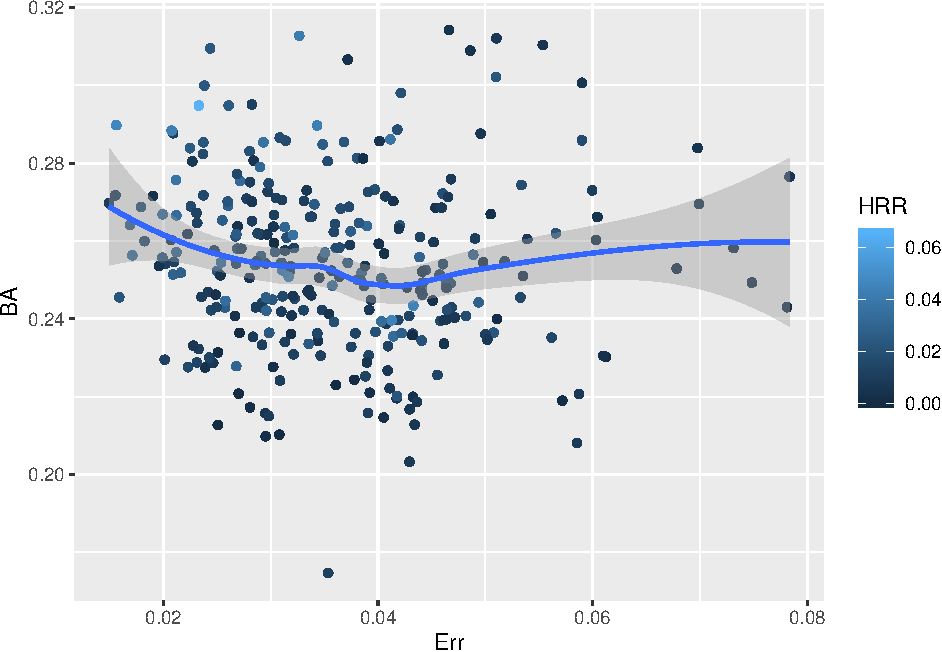
\includegraphics{tidyverse-class_files/figure-latex/ss-stats-1.pdf}

\begin{Shaded}
\begin{Highlighting}[]
\NormalTok{temp <-}\StringTok{ }\NormalTok{batpos }\OperatorTok\StringTok{ }
\StringTok{  }\KeywordTok{mutate}\NormalTok{(}\DataTypeTok{BA =}\NormalTok{ H }\OperatorTok{/}\StringTok{ }\NormalTok{AB) }\OperatorTok\StringTok{  }\CommentTok{# batting average, hits / at bats}
\StringTok{  }\KeywordTok{filter}\NormalTok{(}\KeywordTok{between}\NormalTok{(BA, }\FloatTok{0.01}\NormalTok{, }\FloatTok{0.49}\NormalTok{)) }\OperatorTok\StringTok{ }
\StringTok{  }\KeywordTok{mutate}\NormalTok{(}\DataTypeTok{Err =}\NormalTok{ E }\OperatorTok{/}\StringTok{ }\NormalTok{(PO }\OperatorTok{+}\StringTok{ }\NormalTok{A)) }\OperatorTok\StringTok{   }\CommentTok{# error rate, errors / (put outs + assists)}
\StringTok{  }\KeywordTok{mutate}\NormalTok{(}\DataTypeTok{HRR =}\NormalTok{ HR }\OperatorTok{/}\StringTok{ }\NormalTok{AB)  }\CommentTok{# home run rate, home runs / at bats}
\NormalTok{p1 <-}\StringTok{ }\NormalTok{temp }\OperatorTok\StringTok{ }
\StringTok{  }\KeywordTok{ggplot}\NormalTok{(}\KeywordTok{aes}\NormalTok{(Err, BA, }\DataTypeTok{color =}\NormalTok{ POS)) }\OperatorTok{+}
\StringTok{    }\KeywordTok{geom_point}\NormalTok{(}\DataTypeTok{alpha =} \FloatTok{0.5}\NormalTok{, }\DataTypeTok{size =} \FloatTok{0.5}\NormalTok{) }\OperatorTok{+}
\StringTok{    }\KeywordTok{geom_smooth}\NormalTok{(}\KeywordTok{aes}\NormalTok{(}\DataTypeTok{group =}\NormalTok{ POS)) }\OperatorTok{+}
\StringTok{    }\KeywordTok{coord_cartesian}\NormalTok{(}\DataTypeTok{xlim =} \KeywordTok{c}\NormalTok{(}\DecValTok{0}\NormalTok{, }\FloatTok{0.1}\NormalTok{), }\DataTypeTok{ylim =} \KeywordTok{c}\NormalTok{(}\FloatTok{0.1}\NormalTok{, }\FloatTok{0.42}\NormalTok{))}
\NormalTok{p2 <-}\StringTok{ }\NormalTok{temp }\OperatorTok\StringTok{ }
\StringTok{  }\KeywordTok{filter}\NormalTok{(POS }\OperatorTok{!=}\StringTok{ "P"}\NormalTok{) }\OperatorTok\StringTok{ }
\StringTok{  }\KeywordTok{ggplot}\NormalTok{(}\KeywordTok{aes}\NormalTok{(BA, HRR, }\DataTypeTok{color =}\NormalTok{ POS)) }\OperatorTok{+}
\StringTok{    }\KeywordTok{geom_point}\NormalTok{(}\DataTypeTok{alpha =} \FloatTok{0.5}\NormalTok{, }\DataTypeTok{size =} \FloatTok{0.5}\NormalTok{) }\OperatorTok{+}
\StringTok{    }\KeywordTok{geom_smooth}\NormalTok{(}\KeywordTok{aes}\NormalTok{(}\DataTypeTok{group =}\NormalTok{ POS))}
\NormalTok{p1}
\end{Highlighting}
\end{Shaded}

\begin{verbatim}
## `geom_smooth()` using method = 'loess' and formula 'y ~ x'
\end{verbatim}

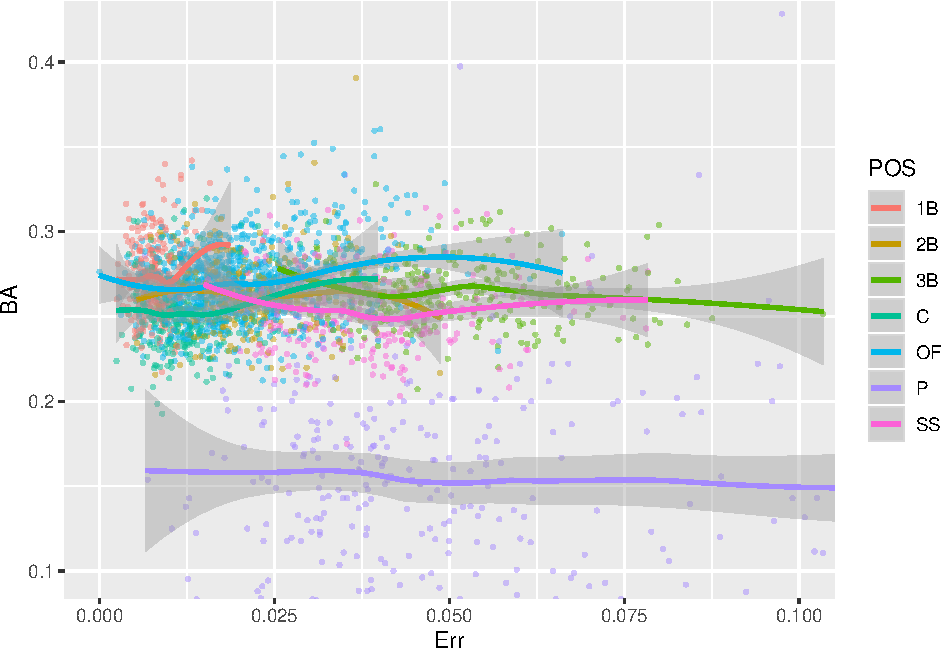
\includegraphics{tidyverse-class_files/figure-latex/plot-pos-ba-1.pdf}

\begin{Shaded}
\begin{Highlighting}[]
\NormalTok{p2}
\end{Highlighting}
\end{Shaded}

\begin{verbatim}
## `geom_smooth()` using method = 'loess' and formula 'y ~ x'
\end{verbatim}

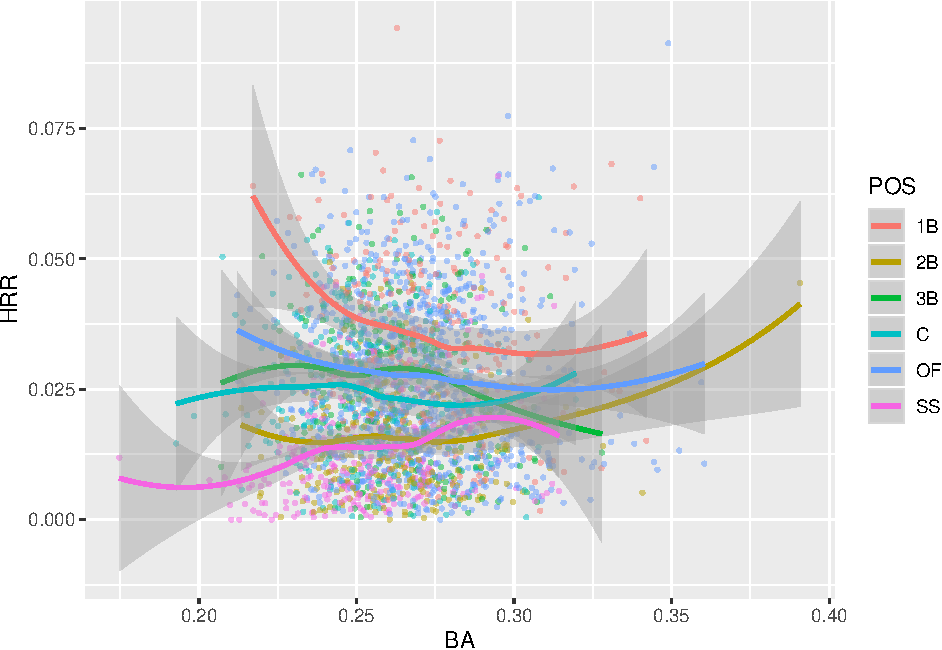
\includegraphics{tidyverse-class_files/figure-latex/plot-pos-ba-2.pdf}

\begin{Shaded}
\begin{Highlighting}[]
\KeywordTok{ggsave}\NormalTok{(}\StringTok{'plots/pos-bat.pdf'}\NormalTok{, }\KeywordTok{arrangeGrob}\NormalTok{(p1, p2))}
\end{Highlighting}
\end{Shaded}

\begin{verbatim}
## Saving 6.5 x 4.5 in image
## `geom_smooth()` using method = 'loess' and formula 'y ~ x'
## `geom_smooth()` using method = 'loess' and formula 'y ~ x'
\end{verbatim}

\bibliography{../clanker.bib,packages.bib}


\end{document}
